\documentclass[11pt,letterpaper]{article}

% ---------- Paquetes ----------
\usepackage[utf8]{inputenc}
\usepackage[T1]{fontenc}
\usepackage[spanish,es-tabla]{babel}
\usepackage[margin=2.5cm]{geometry}
\usepackage{graphicx}
\usepackage{booktabs}
\usepackage{amsmath}
\usepackage{amssymb}
\usepackage{listings}
\usepackage{xcolor}
\usepackage{caption}
\usepackage{hyperref}
\usepackage{enumitem}
\usepackage{float}
% Se agregan nuevos paquetes para arreglar los desbordes
\usepackage[htt]{hyphenat}
\usepackage{seqsplit}

% csquotes no esta disponible en esta instalacion de TeX Live -- se define \enquote a
% mano con el metodo clasico de LaTeX (comilla-comilla de apertura, apostrofe-apostrofe
% de cierre). Evita el conflicto de "..." con los shorthands de babel-spanish (mismo
% bug real encontrado y corregido en docs/ci_cd/informe_ci_cd.tex).
\newcommand{\enquote}[1]{``#1''}

\hypersetup{
    colorlinks=true,
    linkcolor=blue!50!black,
    citecolor=blue!50!black,
    urlcolor=blue!50!black,
    pdftitle={Cierre integral del PFC: aplicaciones web y movil, calidad y evaluacion experimental - Equipo ACC},
    pdfauthor={Carlos Carpio, Cristhian Pacheco, Robinson Cando, Jeremy Alvarez}
}

\definecolor{codebg}{RGB}{245,245,245}
\definecolor{codecomment}{RGB}{100,100,100}
\definecolor{codekeyword}{RGB}{0,0,180}
\definecolor{codestring}{RGB}{160,30,30}

\lstdefinestyle{codigo}{
    backgroundcolor=\color{codebg},
    commentstyle=\color{codecomment}\itshape,
    keywordstyle=\color{codekeyword}\bfseries,
    stringstyle=\color{codestring},
    basicstyle=\footnotesize\ttfamily,
    breakatwhitespace=false,
    breaklines=true,
    captionpos=b,
    keepspaces=true,
    numbers=left,
    numbersep=5pt,
    numberstyle=\tiny\color{codecomment},
    showspaces=false,
    showstringspaces=false,
    showtabs=false,
    tabsize=2,
    frame=single,
    rulecolor=\color{black!20}
}
\lstset{style=codigo}

\title{\textbf{Sistema de Gestión de Solicitudes de Soporte Técnico de Internet}\\
\large Aplicación completa (web y móvil), calidad y evaluación experimental\\
\large Entrega 4 --- Aplicaciones Distribuidas (ISR-701)}

\author{
Carlos Jos\'e Carpio Mendoza \and
Cristhian Daniel Pacheco C\'ardenas \and
Robinson Rodrigo Cando Moreno \and
Jeremy Alexis \'Alvarez P\'arraga\\[1em]
\normalsize Equipo ACC\\
\normalsize Facultad de Ciencias de la Computaci\'on y Dise\~no Gr\'afico\\
\normalsize Carrera de Ingenier\'ia en Software\\
\normalsize Universidad T\'ecnica Estatal de Quevedo
}

\date{Septiembre 2026}

% Entregable 26 de la guia de cierre ("Separacion entre documento vivo y documento congelado"):
% este documento (docs/latex/main.tex) es la fuente viva, recompilada en cada push a main, y no
% puede citar su propio commit sin un problema de huevo-y-gallina (el commit que la crea no
% existe todavia mientras se compila). scripts/congelar_manuscrito.sh reemplaza este mensaje por
% uno especifico de commit+fecha en la copia congelada que produce bajo
% docs/entregas-congeladas/entrega4/ -- ver ese directorio para la version citable de esta
% entrega, no este PDF.
\newcommand{\avisoversion}{Documento vivo: recompilado automáticamente en cada \emph{push} a
\texttt{main}, sin commit ni fecha propios (ver el historial de \texttt{git} de
\texttt{docs/latex/} para saber a qué versión corresponde una compilación dada). Para citar una
versión específica y verificable de esta entrega, use la instantánea congelada en
\texttt{docs/entregas-congeladas/entrega4/} (atada a un commit exacto, con fecha y huella
SHA-256 en su propio \texttt{README.md}).}

\begin{document}

\maketitle

\begin{center}
\fbox{\parbox{0.85\textwidth}{\small \avisoversion}}
\end{center}

\begin{abstract}
\noindent
\textbf{Objetivo.} Cerrar el ciclo del Sistema de Soporte Técnico ISP (equipo ACC) con sus dos
interfaces obligatorias, su capa de calidad automatizada y su evaluación experimental frente a
ISO/IEC 25010:2023~\cite{iso25010}. \textbf{Método.} Se refactorizó el microservicio principal a
arquitectura hexagonal de cuatro capas con seis patrones GoF~\cite{gamma1994patterns},
documentados como ADR con el problema real que resolvían; se construyeron una aplicación web
(React) y una móvil (Kotlin nativo, justificada con dos criterios cuantitativos medidos sobre el
proyecto); se instrumentó el sistema con las tres señales de observabilidad de
OpenTelemetry~\cite{opentelemetry2024spec}; se implementó una pirámide de pruebas completa
(unitarias, integración, contrato con Pact, E2E en tres navegadores, carga con Locust) automatizada
en un pipeline de CI/CD de diez \emph{jobs}; y se midieron cinco características de calidad con
métricas objetivas e intervalos de confianza al 95\,\%. \textbf{Resultados.} El sistema cumple
Compatibilidad (9/9 pruebas E2E en tres navegadores) y Mantenibilidad (96.6\,\% de cobertura de
pruebas y complejidad ciclomática de 1.8, ambos dentro del umbral); Eficiencia y Fiabilidad no
alcanzan su umbral bajo
carga concurrente real, con causa raíz identificada en un límite de licencia del motor de base de
datos, no en la lógica de la aplicación; Seguridad resulta parcialmente mitigada, con una brecha
real documentada (ausencia de protección contra fuerza bruta en el inicio de sesión).
\textbf{Conclusión.} La arquitectura del sistema está diseñada para escalar y es verificable de
extremo a extremo; las brechas encontradas son reales, acotadas y accionables, no ocultadas para
mostrar una nota perfecta.
\end{abstract}

\begin{center}\textbf{Abstract}\end{center}
\begin{abstract}
\noindent
\textbf{Objective.} To close the development cycle of the ISP Technical Support System (team ACC)
with both mandatory client interfaces, an automated quality layer, and an experimental evaluation
against ISO/IEC 25010:2023~\cite{iso25010}. \textbf{Method.} The core microservice was refactored
into a four-layer hexagonal architecture with six GoF patterns~\cite{gamma1994patterns}, each
documented as an ADR against the real design problem it solved; a web client (React) and a native
mobile client (Kotlin, justified with two quantitative criteria measured on the actual project)
were built; the system was instrumented with OpenTelemetry's three observability
signals~\cite{opentelemetry2024spec}; a complete test pyramid (unit, integration, Pact contract,
three-browser E2E, Locust load) was automated in a ten-job CI/CD pipeline; and five quality
characteristics were measured with objective metrics and 95\,\% confidence intervals.
\textbf{Results.} The system meets Compatibility (9/9 E2E tests across three browsers) and
Maintainability (96.6\,\% test coverage and a cyclomatic complexity of 1.8, both within
threshold); Performance
Efficiency and Reliability fall short under real concurrent load, with root cause traced to a
database-engine license limit rather than application logic; Security is partially mitigated,
with one real documented gap (no brute-force protection on login). \textbf{Conclusion.} The
system's architecture is designed to scale and is verifiable end to end; the gaps found are real,
bounded, and actionable, not hidden to present a perfect score.
\end{abstract}


\tableofcontents
\newpage

% ---------- Heredado de E1-E3, sin cambios de estructura ----------
\part{Fundamento heredado (Entregas 1--3)}
\label{part:heredado-e1-e3}
\input{secciones/introduccion}
\input{secciones/trabajos_relacionados}
\input{secciones/fundamento_teorico}
\section{Diseño del esquema y fragmentación}
\label{sec:diseno-esquema}

\subsection{Esquema físico}

La ubicación de la capa de datos dentro de la arquitectura completa del sistema —incluidos el
\texttt{api-gateway}, las aplicaciones cliente y \texttt{telemetry-service}, ya no solo los cinco
microservicios de la Entrega 2— se muestra en la Figura~\ref{fig:c4-nivel2} de la
Sección~\ref{sec:arquitectura-e4}. Esta sección se concentra en el diseño interno de esa capa: la
fragmentación del clúster de CockroachDB (rediseñada en esta entrega) y el pipeline de Spark que
la consume.

El diagrama entidad-relación completo de \texttt{ticket\_db} —la base propia de
\texttt{ticket-service} dentro del clúster de tres nodos de CockroachDB— se documenta en
\texttt{docs/diagrams/db-schema.md}. La tabla \texttt{tickets} es la de mayor cardinalidad y la
única fragmentada; \texttt{technicians} es una dimensión pequeña que no requiere fragmentación. La
Tabla~\ref{tab:esquema-tickets} detalla las columnas relevantes para la política de fragmentación.

\begin{table}[H]
\centering
\caption{Columnas relevantes de \texttt{tickets} tras el rediseño de la Entrega 3}
\label{tab:esquema-tickets}
\begin{tabular}{@{}llp{6.5cm}@{}}
\toprule
\textbf{Columna} & \textbf{Tipo} & \textbf{Rol} \\
\midrule
\texttt{created\_at} & \texttt{TIMESTAMPTZ} & Primer componente de la PK; columna de fragmentación \\
\texttt{id}           & \texttt{UUID}        & Segundo componente de la PK; respaldado además por índice único \texttt{tickets\_id\_key} \\
\texttt{zone}         & \texttt{STRING}      & Columna de negocio (RBAC de técnico, reportes); indexada, ya no es clave de fragmentación \\
\texttt{client\_id}   & \texttt{UUID}        & Identidad del cliente, resuelta a nivel de aplicación vía JWT de \texttt{auth-service} \\
\texttt{status}       & \texttt{STRING}      & Indexada (\texttt{idx\_tickets\_status}) \\
\bottomrule
\end{tabular}
\end{table}

\subsection{Política de fragmentación}

El fragmento del esquema en el Listado~\ref{lst:init-db} muestra la definición efectiva de la
tabla \texttt{tickets} tal como se aplica en la migración Flyway
\texttt{services/svc-principal/.../db/migration/V1\_\_init\_ticket\_schema.sql} (Entregable 5
de la guía de cierre; antes era un guion suelto sin versionar). La verificación de que las
migraciones se aplican de verdad no se limita a \texttt{ticket\_db}: además de
\texttt{TicketRepositoryIntegrationTest} (svc-principal), \texttt{auth-service} y
\texttt{report-service} tienen su propio \texttt{FlywayMigrationIntegrationTest} —cada uno
levanta un CockroachDB real vía Testcontainers, confirma que \texttt{flyway\_schema\_history}
registra la migración V1 como exitosa, y consulta su tabla principal—, en vez de depender solo
del arranque del \emph{stack} completo en el trabajo \texttt{integration} del flujo de CI.

\begin{lstlisting}[language=SQL, caption={Fragmentación por rango de \texttt{tickets} (extracto de \texttt{V1\_\_init\_ticket\_schema.sql})}, label={lst:init-db}]
CREATE TABLE IF NOT EXISTS tickets (
    created_at      TIMESTAMPTZ NOT NULL DEFAULT now(),
    id              UUID NOT NULL DEFAULT gen_random_uuid(),
    zone            STRING NOT NULL,
    client_id       UUID NOT NULL,
    technician_id   UUID REFERENCES technicians(id),
    category        STRING,
    priority        STRING,
    status          STRING NOT NULL DEFAULT 'NUEVO',
    description     STRING,
    sla_deadline    TIMESTAMPTZ,
    resolved_at     TIMESTAMPTZ,
    sla_breached    BOOL DEFAULT FALSE,
    PRIMARY KEY (created_at, id)
) PARTITION BY RANGE (created_at) (
    PARTITION tickets_2026_q1 VALUES FROM (MINVALUE) TO ('2026-04-01T00:00:00Z'),
    PARTITION tickets_2026_q2 VALUES FROM ('2026-04-01T00:00:00Z') TO ('2026-07-01T00:00:00Z'),
    PARTITION tickets_2026_q3 VALUES FROM ('2026-07-01T00:00:00Z') TO ('2026-10-01T00:00:00Z'),
    PARTITION tickets_2026_q4 VALUES FROM ('2026-10-01T00:00:00Z') TO (MAXVALUE)
);

CREATE UNIQUE INDEX IF NOT EXISTS tickets_id_key ON tickets (id);
CREATE INDEX IF NOT EXISTS idx_tickets_zone ON tickets (zone);
CREATE INDEX IF NOT EXISTS idx_tickets_status ON tickets (status);
\end{lstlisting}

Esta sintaxis sigue el mecanismo de particionamiento declarativo documentado oficialmente por
Cockroach Labs~\cite{cockroachlabs2024docs}, que exige que la columna de partición sea el primer
componente de la clave primaria para que el optimizador pueda aplicar poda de particiones
(\emph{partition pruning}) en tiempo de planificación de consultas. Esta decisión reemplaza el
diseño original de la Entrega 2, que fragmentaba \texttt{tickets} por
zona geográfica (\texttt{PARTITION BY LIST (zone)}). El cambio fue motivado por un requisito
explícito y no negociable de la guía oficial de la Entrega 3 para el equipo ACC: fragmentación
horizontal de \texttt{tickets} por \texttt{fecha\_apertura}. El razonamiento completo de este
cambio, incluyendo los \emph{trade-offs} aceptados, se documenta en el ADR-0003
(\texttt{docs/adr/0003-sharding-policy.md}) y se resume a continuación.

\subsection{Verificación formal de corrección}

Con $a = \texttt{created\_at}$ y los cuatro puntos de corte del Listado~\ref{lst:init-db}
($c_0 = \text{MINVALUE}$, $c_1 = \text{2026-04-01}$, $c_2 = \text{2026-07-01}$,
$c_3 = \text{2026-10-01}$, $c_4 = \text{MAXVALUE}$), se verifican las tres condiciones del
marco de Özsu y Valduriez~\cite{ozsu2011principles} introducidas en la
Sección~\ref{sec:fundamento-teorico}:

\begin{itemize}[leftmargin=1.5em]
    \item \textbf{Completitud}: la columna \texttt{created\_at} es \texttt{NOT NULL} con valor
        por defecto \texttt{now()}, por lo que todo ticket tiene un valor definido de
        \texttt{created\_at} y, en consecuencia, pertenece a exactamente una de las cuatro
        particiones trimestrales.
    \item \textbf{Reconstrucción}: los rangos
        $[\text{MINVALUE}, c_1) \cup [c_1, c_2) \cup [c_2, c_3) \cup [c_3, \text{MAXVALUE})$
        cubren la totalidad del dominio de \texttt{TIMESTAMPTZ}; la unión \texttt{UNION ALL} de
        las cuatro particiones reconstruye exactamente la tabla \texttt{tickets} sin pérdida de
        filas.
    \item \textbf{Disyunción}: la semántica de \texttt{PARTITION BY RANGE} en CockroachDB define
        cada límite como inclusivo por la izquierda y exclusivo por la derecha
        (\texttt{VALUES FROM ... TO ...}); por construcción, ningún valor de \texttt{created\_at}
        satisface simultáneamente los predicados de dos particiones distintas.
\end{itemize}

Adicionalmente, dado que \texttt{id} deja de ser autosuficiente como punto de acceso —la
aplicación recibe un UUID de ticket sin conocer su \texttt{created\_at} de antemano en los
\emph{endpoints} \texttt{GET}/\texttt{PATCH} sobre \texttt{/api/v1/tickets/\{id\}}—, se añadió el índice único secundario
\texttt{tickets\_id\_key}, usado por \texttt{TicketRepository.findByTicketId(UUID)} para resolver
ese acceso con un único salto índice→tabla, sin necesidad de escanear las cuatro particiones.

\subsection{Colocalización con clientes y limitación arquitectónica}

La guía de la Entrega 3 pide, además de la fragmentación por fecha, colocalizar \texttt{tickets}
con \texttt{clientes} por \texttt{client\_id}, lo que en CockroachDB se implementaría típicamente
con \texttt{INTERLEAVE IN PARENT} o una clave compartida dentro de la misma base de datos. En la
arquitectura de microservicios heredada de la Entrega 2, los clientes son propiedad exclusiva de
\texttt{auth-service} (\texttt{auth\_db.users}), una base de datos físicamente distinta de
\texttt{ticket\_db} — cada microservicio es dueño de su propio esquema, sin acceso cruzado directo
a la base de otro. Forzar una colocalización física en el sentido literal de CockroachDB
requeriría fusionar ambas bases de datos, violando el límite de propiedad de datos entre servicios
que es una decisión arquitectónica deliberada, no un descuido, de la Entrega 2. Se documenta esta
tensión explícitamente en el ADR-0003 en vez de forzar una colocalización artificial: la columna
\texttt{tickets.client\_id} permanece indexada para soportar las consultas
\texttt{findByClientId}/\texttt{findByClientIdAndStatus}, y la resolución de identidad del cliente
ocurre a nivel de aplicación mediante el JWT emitido por \texttt{auth-service}, no a nivel de
almacenamiento físico compartido.

\subsection{Política de replicación}

Como la fragmentación pasó de ser por zona a ser por fecha, ya no existe una correspondencia 1:1
entre una partición y la \emph{locality} de un nodo específico: una partición trimestral contiene
tickets de las tres zonas geográficas mezclados. En consecuencia, la política de replicación
(Listado~\ref{lst:zones}) ya no ancla particiones a nodos por restricción de \emph{locality};
exige uniformemente un factor de replicación 3 sobre toda la tabla, de forma que la pérdida de
cualquier nodo individual del clúster de tres no comprometa la disponibilidad de escritura
(2 de 3 réplicas siguen constituyendo mayoría para Raft~\cite{ongaro2014raft}). Al igual que el
esquema de la Sección anterior, esta política es hoy la migración Flyway
\texttt{V2\_\_configure\_ticket\_zone.sql} (Entregable 5 de la guía de cierre), aplicada
automáticamente después de \texttt{V1} en vez del guion suelto \texttt{db-cluster/config/zones.sql}
que existía hasta entonces —ese archivo se retiró del repositorio, no quedó como una segunda
copia que pudiera desincronizarse de la migración real.

\begin{lstlisting}[language=SQL, caption={Política de replicación uniforme (\texttt{V2\_\_configure\_ticket\_zone.sql})}, label={lst:zones}]
ALTER TABLE tickets CONFIGURE ZONE USING num_replicas = 3;
\end{lstlisting}

\subsection{Trade-offs aceptados}

El rediseño no es gratuito: las consultas filtradas por zona —el filtro más frecuente en la
operación real de un ISP, usado por el RBAC de técnico y por la mayoría de los reportes— dejan de
beneficiarse de poda de particiones y pasan a resolverse mediante \emph{scatter-gather} sobre las
cuatro particiones trimestrales, mientras que antes se resolvían dentro de una sola partición. Este
\emph{trade-off}, junto con el beneficio simétrico obtenido por las consultas de rango temporal
(la mayoría de los reportes reales: ``tickets abiertos hoy'', ``tickets del último trimestre''), se
mide de forma comparativa con \texttt{EXPLAIN ANALYZE} sobre las cinco consultas representativas de
\texttt{db-cluster/scripts/queries\_bench.sql} (lectura por \texttt{id}, rango de fecha, filtro por
zona, agregación de incumplimiento de SLA, y \emph{join} con técnicos), documentadas junto con sus
planes de ejecución en el Anexo correspondiente del repositorio.

\section{Cluster y su verificación}
\label{sec:cluster-verificacion}

\subsection{Levantamiento del clúster de tres nodos}

El clúster se define en \texttt{db-cluster/docker-compose.cockroach.yml} con tres servicios
(\texttt{roach1}, \texttt{roach2}, \texttt{roach3}) sobre la red \texttt{bridge}
\texttt{soporte-net}, cada uno con volumen persistente propio y el comando
\texttt{start --insecure --join=roach1,roach2,roach3} apuntando al resto de nodos —siguiendo el
patrón estándar de arranque de un clúster CockroachDB multi-nodo. Cada nodo declara además una
\texttt{locality} distinta (\texttt{quevedo-centro}, \texttt{quevedo-norte},
\texttt{quevedo-sur}), simulando las tres zonas operativas del ISP para fines de política de
replicación, y expone un \emph{healthcheck} HTTP sobre \texttt{/health?ready=1} que Docker Compose
usa para reportar el estado del contenedor.

\begin{lstlisting}[language=bash, caption={Extracto de \texttt{docker-compose.cockroach.yml}: definición de un nodo}, label={lst:compose-crdb}]
roach1:
  image: cockroachdb/cockroach:latest-v23.2
  command: start --insecure --max-offset=4500ms
    --locality=zone=quevedo-centro
    --join=roach1,roach2,roach3
  ports: ["26257:26257", "8083:8080"]
  volumes: ["roach1-data:/cockroach/cockroach-data"]
  networks: [soporte-net]
\end{lstlisting}

Tras \texttt{docker compose -f docker-compose.cockroach.yml up -d}, el clúster se inicializa una
única vez con \texttt{cockroach init --insecure} ejecutado contra cualquiera de los tres nodos.
La verificación de que los tres nodos forman efectivamente un único clúster operativo se realiza
con \texttt{cockroach node status --insecure}, que debe reportar los tres identificadores de nodo
con \texttt{is\_live=true} e \texttt{is\_available=true}; el mismo estado es visible en la consola
web del clúster (puerto 8083 en este despliegue, reasignado desde el 8080 por defecto para no
chocar con otro servicio local). Sobre este clúster ya verificado operativo se aplica el esquema
fragmentado descrito en la Sección~\ref{sec:diseno-esquema} y se ejecutan las pruebas de
integración y la instrumentación de métricas de las siguientes subsecciones.

\subsection{Pruebas de integración contra CockroachDB real}

Para evitar que la corrección del acceso a datos dependiera únicamente de pruebas unitarias con
\emph{mocks} —que no pueden reproducir comportamiento específico de CockroachDB como el
aislamiento \texttt{SERIALIZABLE} o los tipos nativos \texttt{UUID}/\texttt{STRING}—, se añadió una
suite de pruebas de integración basada en Testcontainers
(\texttt{TicketRepositoryIntegrationTest.java}) que levanta un contenedor real de
\texttt{cockroachdb/cockroach:latest-v23.2} en modo \texttt{start-single-node} para cada ejecución
de la suite y lo descarta automáticamente al finalizar (limpieza gestionada por el
\emph{sidecar} Ryuk de Testcontainers, sin intervención manual). El esquema ya no lo crea la
prueba a mano: con \texttt{flyway-core} en el \emph{classpath}, Spring Boot aplica
automáticamente la migración real
\texttt{V1\_\_init\_ticket\_schema.sql} (Entregable 5 de la guía de cierre) contra esa misma base
al construir el contexto de la aplicación —el guion suelto \texttt{db-cluster/scripts/init\_db.sql}
que esta prueba citaba antes de esa corrección ya no existe en el repositorio, precisamente para
que una migración rota se detecte aquí en vez de poder divergir en silencio de un guion aparte.

La suite contiene dos pruebas. La primera ejerce el mismo \texttt{TicketRepository} usado en
producción con una operación real de guardado y búsqueda por \texttt{findByTicketId(UUID)} —el
mismo camino que ejercita el índice único secundario \texttt{tickets\_id\_key} descrito en la
Sección~\ref{sec:diseno-esquema}—. La segunda es una prueba empírica, no simulada, de que el
clúster aplica de verdad aislamiento \texttt{SERIALIZABLE}: dos hilos abren cada uno su propia
conexión y transacción, ambos leen la misma fila de \texttt{tickets} (sincronizados con una
barrera para garantizar que ambas lecturas ocurren antes de cualquier escritura) y luego ambos
intentan actualizar el mismo campo \texttt{status}. El resultado esperado —y observado— es que al
menos una de las dos transacciones falle al hacer \texttt{commit} con un error de conflicto de
escritura serializable, identificado por el código de estado SQL \texttt{40001}:

\begin{lstlisting}[language=Java, caption={Extracto de la prueba de conflicto serializable}, label={lst:testcontainers}]
assertThat((Exception) conflict.get())
    .describedAs("al menos una de las dos transacciones concurrentes "
        + "debio fallar por conflicto serializable")
    .isNotNull();
assertThat(conflict.get().getSQLState()).isEqualTo("40001");
\end{lstlisting}

Esta prueba corrobora en código, de forma reproducible en cualquier máquina con Docker
(incluyendo el entorno de integración continua), el mismo tipo de error observado en producción
en \texttt{report-service} (\texttt{ReportEventListener.applyWithRetry}) y que
\texttt{TicketService} está preparado para reintentar automáticamente (ver
Sección~\ref{sec:cluster-verificacion}, métricas de reintento). Ambas pruebas se ejecutaron de
forma exitosa contra la imagen real de CockroachDB antes de la integración de esta sección.

\subsection{Instrumentación de métricas operativas}

\texttt{ticket-service} expone tres métricas Prometheus, registradas mediante Micrometer y
consumibles en el \emph{endpoint} \texttt{/actuator/prometheus}, descritas en la
Tabla~\ref{tab:metricas}.

\begin{table}[H]
\centering
\caption{Métricas Prometheus expuestas por \texttt{ticket-service}}
\label{tab:metricas}
\begin{tabular}{@{}p{4.3cm}p{1.8cm}p{6.7cm}@{}}
\toprule
\textbf{Métrica} & \textbf{Tipo} & \textbf{Significado} \\
\midrule
\texttt{crdb\_query\_duration\_seconds} & Histograma & Duración de cada consulta a \texttt{TicketRepository}, con histograma de percentiles \\
\texttt{crdb\_transaction\_retries\_total} & Contador & Reintentos por conflicto de escritura serializable \\
\texttt{crdb\_pool\_active\_connections} & \emph{Gauge} & Conexiones activas del \emph{pool} HikariCP hacia CockroachDB \\
\bottomrule
\end{tabular}
\end{table}

El histograma de duración se alimenta desde un \emph{aspect} de Spring AOP
(\texttt{RepositoryTimingAspect}) que envuelve cada llamada al repositorio sin requerir
instrumentación manual en cada método de servicio. El contador de reintentos se incrementa
explícitamente desde \texttt{TicketService} cada vez que una operación de guardado captura una
\texttt{ConcurrencyFailureException} y reintenta —el mismo mecanismo ejercitado por la prueba de
conflicto serializable de la subsección anterior—. El \emph{gauge} de conexiones activas no
mantiene un valor cacheado: Micrometer lo reconsulta bajo demanda directamente contra el
\texttt{HikariPoolMXBean} real del \emph{pool}, por lo que siempre refleja el estado actual del
\emph{pool}, no una fotografía tomada en el momento del registro.

Las tres métricas se validaron con el \emph{linter} oficial de Prometheus (\texttt{promtool check
metrics}) ejecutado sobre la salida cruda del \emph{endpoint}, dentro de un contenedor
\texttt{prom/prometheus:latest} para no requerir una instalación local de Prometheus. La
validación no reportó advertencias ni errores sobre los tres instrumentos: los nombres siguen la
convención de sufijo por unidad (\texttt{\_seconds}, \texttt{\_total}), y las descripciones
(\texttt{HELP}) y tipos (\texttt{TYPE}) están correctamente declarados en la exposición.

\subsection{Tolerancia a fallos del clúster}

El protocolo de medición de tolerancia a fallos consiste en generar una carga de escritura
sostenida contra el clúster de tres nodos, derribar deliberadamente un nodo
(\texttt{docker stop roach2}) y registrar la latencia P50/P95 de las operaciones de escritura
antes, durante y después de la caída, repitiendo después el mismo procedimiento derribando dos
nodos simultáneamente para observar la pérdida de disponibilidad de escritura predicha por la
teoría de consenso de la Sección~\ref{sec:fundamento-teorico} (con dos de tres nodos caídos ya no
existe mayoría para confirmar escrituras vía Raft).

Durante la preparación de este protocolo se recreó, de forma no planificada pero informativa, el
escenario adyacente de saturación de memoria: una carga inicial de 150{,}000 filas en una sola
transacción provocó que el nodo \texttt{roach1} fuera terminado por el sistema operativo por falta
de memoria (código de salida 137) bajo el límite original de 512\,MB por contenedor, y el propio
reinicio del nodo —una operación intensiva en memoria en CockroachDB, que debe reconstruir su
estado desde el registro de Raft— volvió a fallar por el mismo motivo antes de estabilizarse. El
límite de memoria de los tres nodos se incrementó a 1024\,MB en
\texttt{docker-compose.cockroach.yml} como mitigación documentada, y la recarga completa del
conjunto de datos de 150{,}000 filas se replanificó en lotes más pequeños para el protocolo formal
de tolerancia a fallos. Este incidente, aunque no forma parte del protocolo experimental
diseñado, es evidencia operativa consistente con la teoría: un nodo bajo presión de recursos deja
de poder participar en el consenso, degradando la disponibilidad del clúster de la misma forma
que una caída deliberada, y su recuperación no es instantánea.

\subsubsection{Resultados}

El protocolo se ejecutó con una carga inicial de 101{,}996 filas en \texttt{tickets}. La
Tabla~\ref{tab:tolerancia-1nodo} resume la carga sostenida (\texttt{load\_write.py},
100 filas/s) durante la caída de \texttt{roach2}.

\begin{table}[H]
\centering
\caption{Latencia por ventana de 10s durante la caída de 1 nodo (roach2)}
\label{tab:tolerancia-1nodo}
\begin{tabular}{@{}lrrrr@{}}
\toprule
\textbf{Ventana} & \textbf{P50} & \textbf{P95} & \textbf{Errores} & \textbf{Filas} \\
\midrule
1 & 38.6 ms & 118.4 ms & 0 & 110 \\
2 (\texttt{docker kill roach2}) & 69.3 ms & \textbf{1590.8 ms} & 0 & 44 \\
3 & 31.0 ms & 107.9 ms & 0 & 130 \\
4 & 40.2 ms & 95.7 ms & 0 & 114 \\
5 & 26.3 ms & 69.3 ms & 0 & 163 \\
\bottomrule
\end{tabular}
\end{table}

El pico de $P95=1590.8$\,ms en la ventana 2 coincide con el instante de \texttt{docker kill
roach2}: el tiempo que Raft necesita para reelegir líder en los rangos cuyo \emph{leaseholder} era
roach2. Ningún dato se pierde ni falla (0 errores en las 691 filas insertadas); el único efecto
observable es latencia transitoria, no indisponibilidad — el clúster tolera la caída de un nodo
sin degradar la disponibilidad de escritura, como predice el quórum de mayoría 2 de 3.

Al repetir la prueba derribando también \texttt{roach3} (solo \texttt{roach1} en pie), la carga
sostenida (50 filas/s) muestra una brecha de \textbf{62 segundos} entre dos ventanas consecutivas
que normalmente distan 10-12\,s, coincidiendo exactamente con la ventana de tiempo en la que
ambos nodos permanecieron caídos: sin mayoría posible, la conexión abierta quedó bloqueada
esperando confirmación en vez de recibir un error inmediato, y una consulta
\texttt{SELECT count(*)} lanzada en ese mismo intervalo no devolvió resultado hasta reincorporar
\texttt{roach2}. Esta indisponibilidad por bloqueo —en vez de una excepción explícita del
cliente— es una manifestación válida de la pérdida de disponibilidad de escritura predicha por la
teoría de consenso: con un solo nodo vivo de tres no existe mayoría para que Raft confirme ninguna
escritura, exactamente el límite documentado en la Sección~\ref{sec:fundamento-teorico}. La
recuperación es inmediata al ejecutar \texttt{docker start roach2}: con dos nodos vivos vuelve a
haber quórum y la latencia regresa a valores normales (20.6/43.9\,ms). El detalle completo,
incluyendo la secuencia exacta de comandos, está en la bitácora
(\texttt{docs/evidencias/tolerancia\_fallos.md}) y el video
(\texttt{docs/evidencias/tolerancia\_fallos.mp4}, 4:55~min).

\begin{figure}[H]
\centering
\includegraphics[width=0.8\textwidth]{figuras/consola-recuperacion.jpg}
\caption{Consola web de CockroachDB tras la recuperación final: los tres nodos en estado
\texttt{LIVE}, 61 réplicas cada uno (captura del video de tolerancia a fallos).}
\label{fig:consola-recuperacion}
\end{figure}

\input{secciones/pipeline_paralelo}
\input{secciones/protocolo_resultados}

% ---------- Nuevo de la Entrega 4 ----------
\part{Aportes de la Entrega 4}
\label{part:aportes-e4}
\input{secciones/fundamento_teorico_e4}
\section{Arquitectura del sistema}
\label{sec:arquitectura-e4}

Esta sección documenta la arquitectura resultante tras la Entrega 4 en los tres niveles del
modelo C4~\cite{brown2018c4model}, y resume las decisiones registradas como \emph{Architectural
Decision Records} (ADR) que la sustentan.

\subsection{Vista de contexto (C4 Nivel 1)}

La Figura~\ref{fig:c4-nivel1} sitúa el sistema como una sola caja frente a sus tres tipos de
usuario. No hay sistemas externos reales que integrar en este nivel: lo que podría parecer una
integración externa —notificaciones multicanal, telemetría de equipos del abonado— está simulado
dentro del propio sistema y documentado como tal en cada ADR correspondiente (ver
\texttt{docs/diagrams/c4-nivel1-contexto.md} para el detalle de por qué).

\begin{figure}[H]
\centering
\includegraphics[width=0.85\textwidth]{../diagrams/c4-nivel1-contexto.png}
\caption{C4 Nivel 1 — contexto del sistema.}
\label{fig:c4-nivel1}
\end{figure}

\subsection{Vista de contenedores (C4 Nivel 2)}

El diagrama de contenedores de la Entrega 3 (\texttt{docs/diagrams/c4-nivel2-contenedores.md})
se actualiza en esta entrega con las piezas nuevas: las dos
aplicaciones cliente (\texttt{apps/web}, \texttt{apps/mobile}) ya no hablan directamente con cada
microservicio por su puerto, sino que pasan por un único \texttt{api-gateway} (Spring Cloud
Gateway) que enruta por prefijo de \emph{path} sin reescribir el cuerpo de la petición. Se agrega
\texttt{telemetry-service} (PE-U1, Sección~\ref{sec:pe-u1-correl}) como séptimo microservicio, y
el stack de observabilidad (OpenTelemetry Collector, Tempo, Prometheus, Grafana, cAdvisor) como
un grupo de contenedores transversal. La Figura~\ref{fig:c4-nivel2} muestra el diagrama completo.

\begin{figure}[H]
\centering
\includegraphics[width=\textwidth,height=0.92\textheight,keepaspectratio]{../diagrams/c4-nivel2-contenedores.png}
\caption{C4 Nivel 2 — contenedores del sistema, Entrega 4.}
\label{fig:c4-nivel2}
\end{figure}

\begin{table}[H]
\centering
\small
\caption{Contenedores del sistema tras la Entrega 4.}
\label{tab:contenedores-e4}
\begin{tabular}{@{}p{3.1cm}p{2.6cm}p{7.8cm}@{}}
\toprule
\textbf{Contenedor} & \textbf{Tecnología} & \textbf{Responsabilidad} \\
\midrule
\texttt{apps/web} & React 18 + TypeScript & SPA de consola para clientes/técnicos/administradores \\
\texttt{apps/mobile} & Kotlin + Jetpack Compose & Cliente de campo para técnicos (APK) \\
\texttt{api-gateway} & Spring Cloud Gateway & Único punto de entrada, enrutamiento por prefijo \\
\texttt{auth-service} & Java 21 + Spring Boot & JWT, RBAC, refresh tokens \\
\texttt{ticket-service} & Java 21 + Spring Boot & CRUD de tickets, arquitectura hexagonal (Sección~\ref{sec:hexagonal-e4}) \\
\texttt{ai-service} & Python + FastAPI & Clasificación asíncrona por reglas \\
\texttt{notification-service} & Node.js + Express & Notificaciones multicanal simuladas \\
\texttt{report-service} & Java 21 + Spring Boot & Modelo de lectura CQRS, reportes \\
\texttt{telemetry-service} & Java 21, sockets TCP + gRPC & Canal PE-U1: equipos del abonado + latidos de nodo, reloj de Lamport (Sección~\ref{sec:pe-u1-correl}) \\
CockroachDB & Cluster 3 nodos & Persistencia distribuida (auth\_db/ticket\_db/report\_db) \\
Kafka + MongoDB & --- & Saga por coreografía, clasificaciones y notificaciones \\
OTel Collector, Tempo, Prometheus, Grafana, cAdvisor & --- & Observabilidad (Sección~\ref{sec:observabilidad}) \\
\bottomrule
\end{tabular}
\end{table}

\subsection{Vista de componentes (C4 Nivel 3)}
\label{sec:c4-nivel3}

El único servicio con arquitectura hexagonal completa es \texttt{ticket-service}
(Sección~\ref{sec:hexagonal-e4}), así que es el que se documenta en este nivel del modelo:
zoom a sus componentes reales, no a una aproximación. La Figura~\ref{fig:c4-nivel3} —fuente
versionada en \texttt{docs/diagrams/c4-nivel3-componentes.md}— nombra cada caja igual que el
árbol de \texttt{services/svc-principal/src/main/java/.../ticketservice/}: los seis patrones GoF
de la Sección~\ref{sec:gof-e4} son visibles aquí, no solo enumerados en prosa.

La imagen fuente (\texttt{docs/diagrams/c4-nivel3-componentes.png}) es extremadamente alargada
(1109×4348~px, relación de aspecto 1:4) porque Mermaid apila las 27 cajas en una sola columna
vertical. Encajada como una sola figura en una página vertical (con la altura acotada al 85\,\% de la
altura de página), el ancho resultante quedaba en apenas ~5~cm, con el texto de cada caja en torno a 1,4~pt
impreso —ilegible, aunque la imagen en sí no perdiera contenido— (hallazgo de una revisión
externa). Se divide aquí en cuatro franjas horizontales iguales, de arriba a abajo, sin recortar
ni omitir ninguna caja, dispuestas en una cuadrícula de $2\times2$ para que cada franja quede
acotada por el ancho de página (el lado que faltaba aprovechar) en vez de por la altura:

\begin{figure}[H]
\centering
\begin{minipage}{0.48\textwidth}
  \centering
  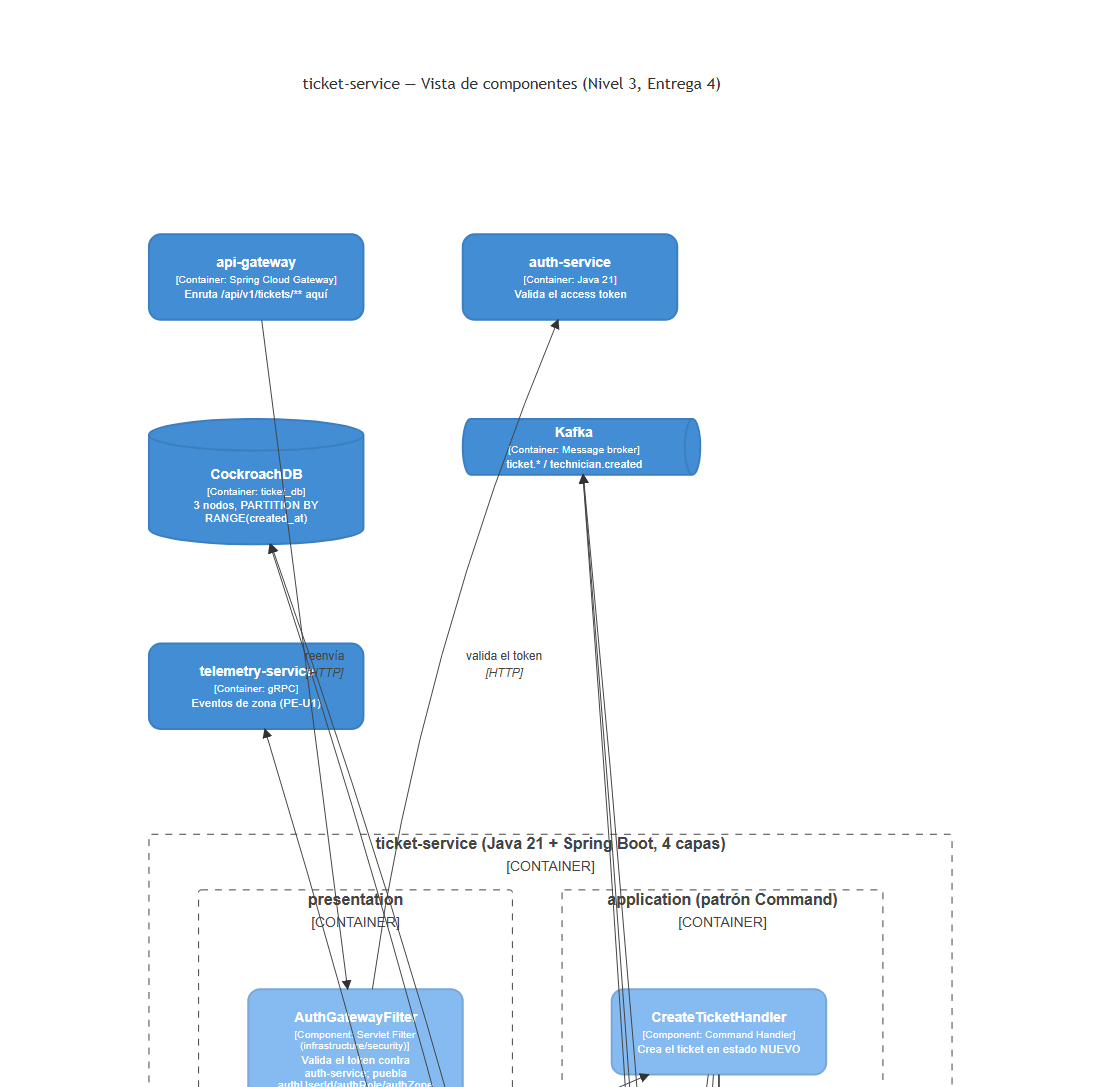
\includegraphics[width=\linewidth]{../diagrams/c4-nivel3-componentes-parte1.png}
  \\ \footnotesize (a)
\end{minipage}
\hfill
\begin{minipage}{0.48\textwidth}
  \centering
  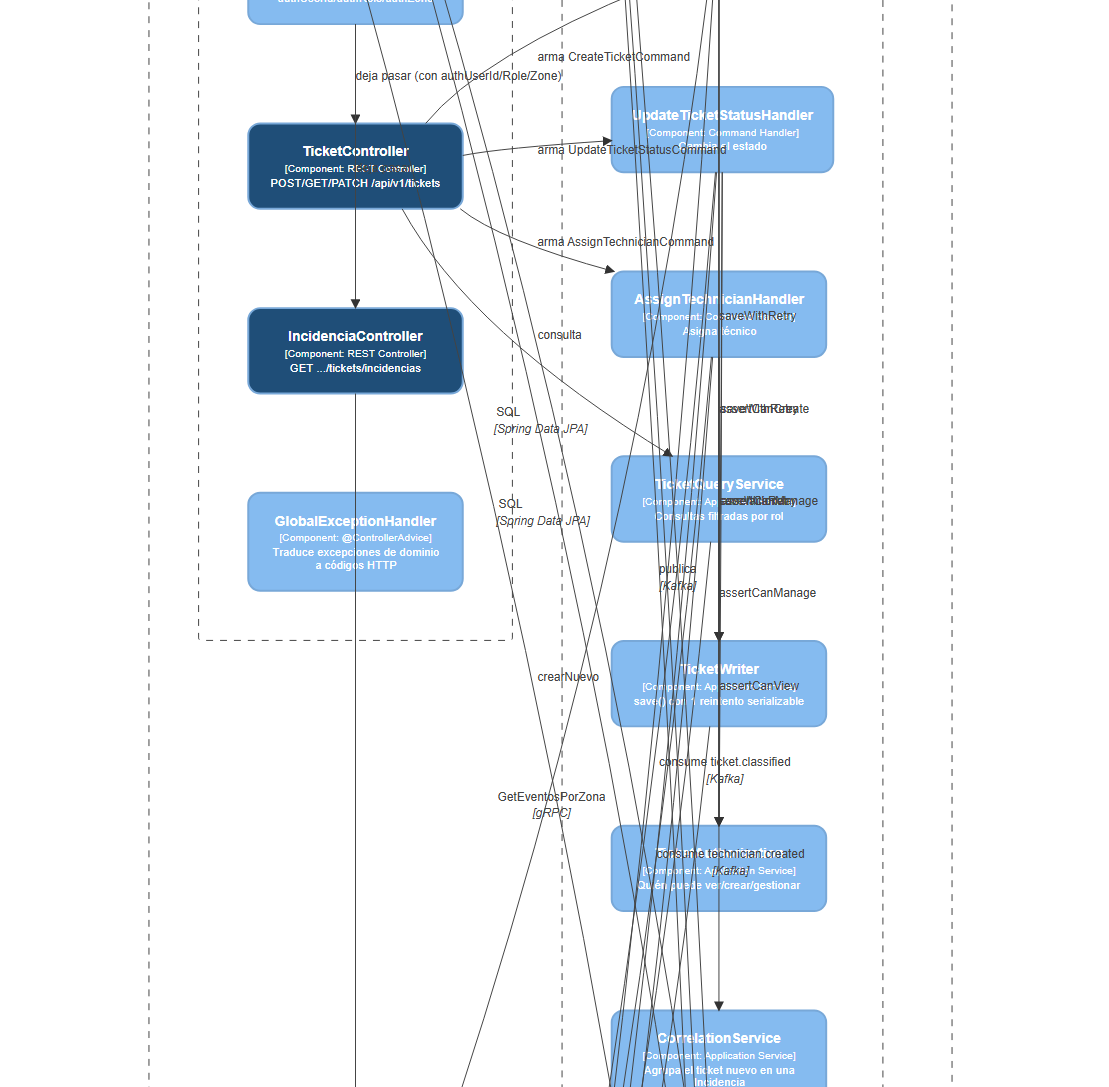
\includegraphics[width=\linewidth]{../diagrams/c4-nivel3-componentes-parte2.png}
  \\ \footnotesize (b)
\end{minipage}

\vspace{4pt}
\begin{minipage}{0.48\textwidth}
  \centering
  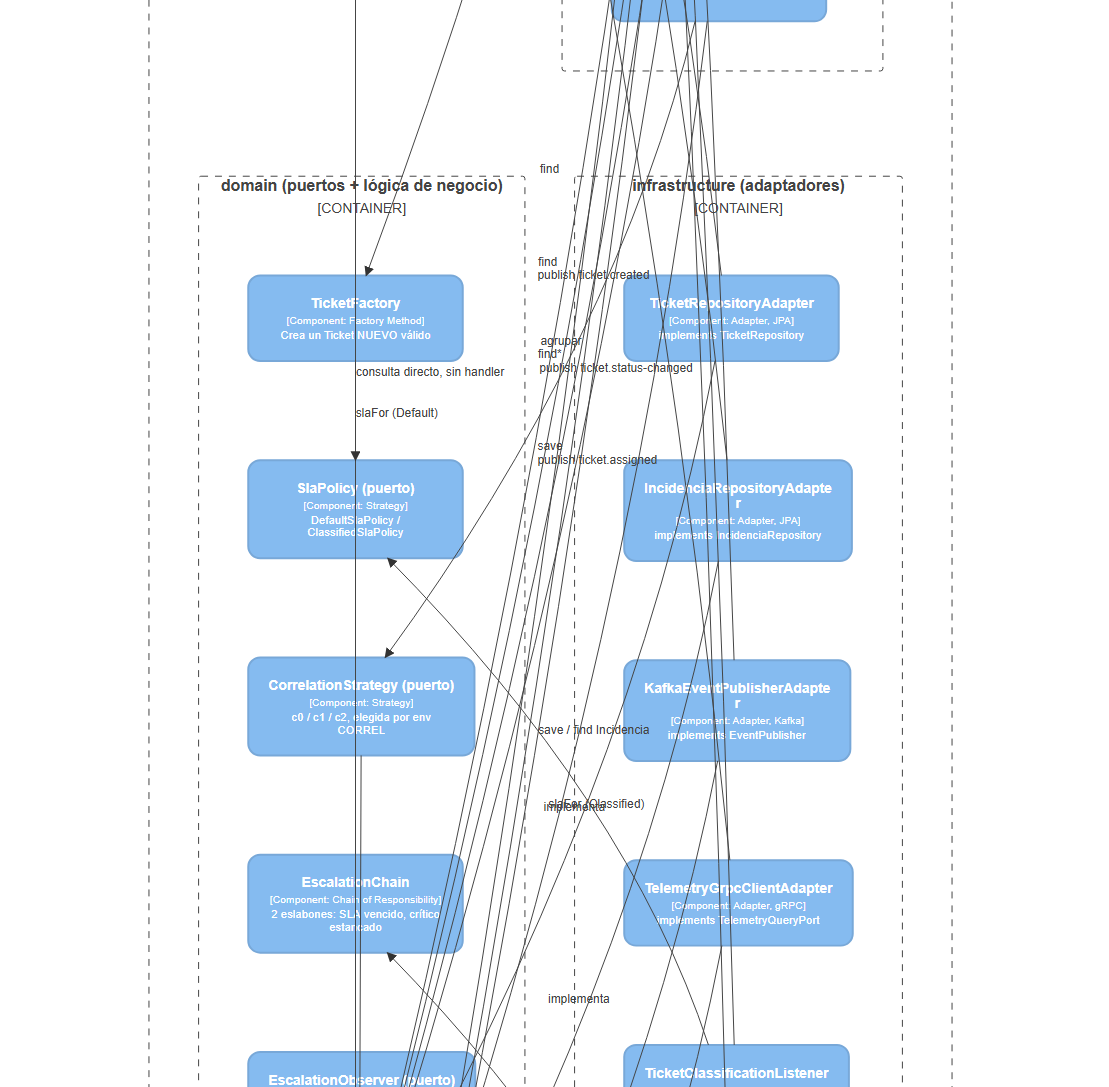
\includegraphics[width=\linewidth]{../diagrams/c4-nivel3-componentes-parte3.png}
  \\ \footnotesize (c)
\end{minipage}
\hfill
\begin{minipage}{0.48\textwidth}
  \centering
  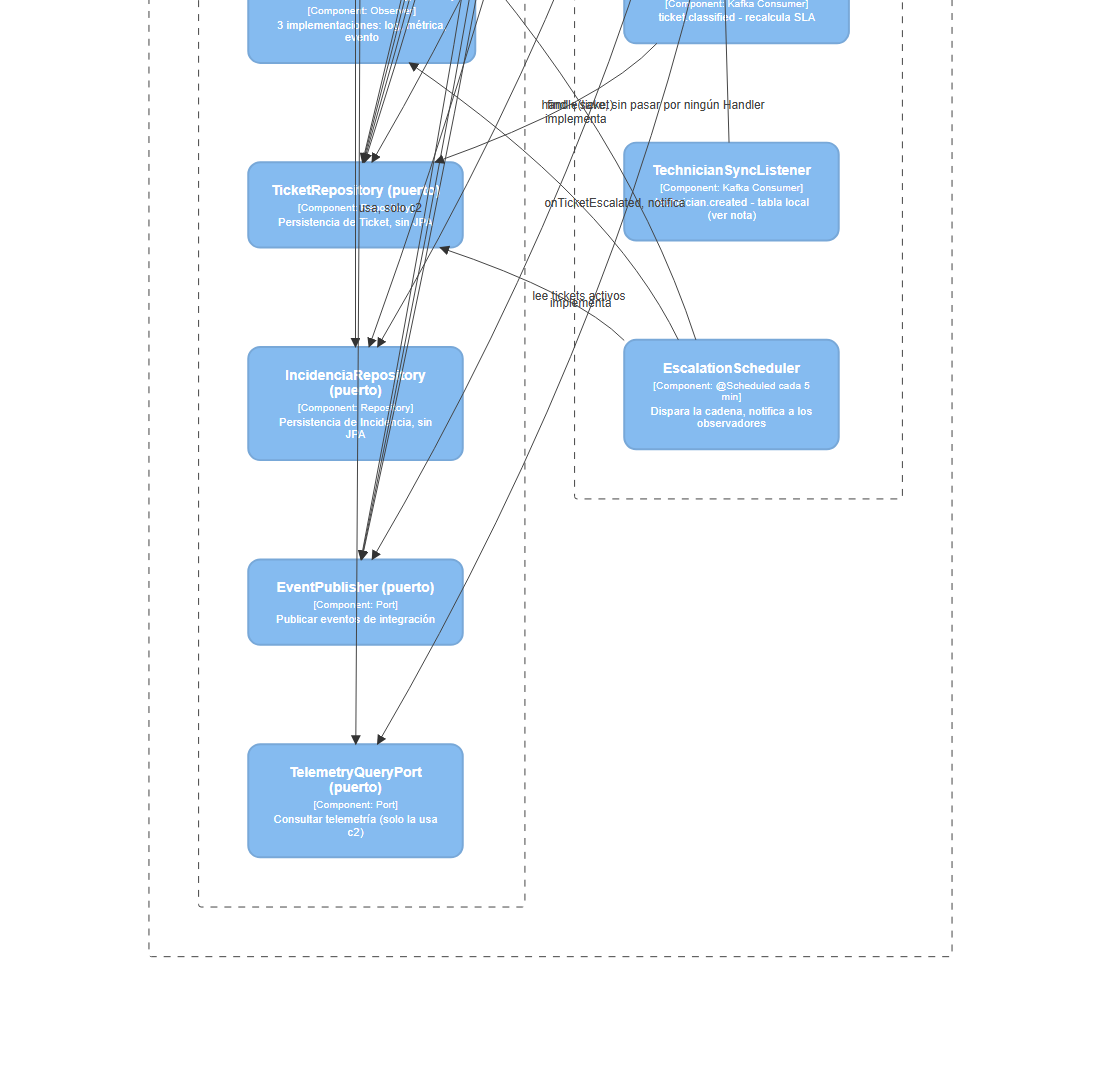
\includegraphics[width=\linewidth]{../diagrams/c4-nivel3-componentes-parte4.png}
  \\ \footnotesize (d)
\end{minipage}
\caption{C4 Nivel 3 — componentes de \texttt{ticket-service}, Entrega 4. Mismo diagrama que
\texttt{c4-nivel3-componentes.png}, dividido en cuatro franjas horizontales (a)--(d), de arriba
a abajo, para que el texto de cada caja sea legible en la página.}
\label{fig:c4-nivel3}
\end{figure}

Dos rutas del diagrama rompen deliberadamente la capa de aplicación, documentado en vez de
ocultado: \texttt{IncidenciaController} consulta \texttt{IncidenciaRepository} directo (es una
lectura simple, sin caso de uso que orquestar), y \texttt{TicketClassificationListener} opera
sobre \texttt{TicketRepository} sin pasar por ningún \texttt{*CommandHandler} (el caso de uso
real es aplicar una clasificación asíncrona llegada por Kafka, no una acción HTTP con
autorización de rol). \texttt{TechnicianSyncListener} tampoco tiene puerto de dominio: escribe
directo en una tabla de sincronización local que no representa un concepto propio de
\texttt{ticket-service} --es una réplica de solo lectura de datos de \texttt{auth-service},
necesaria para que \texttt{AssignTechnicianHandler} no viole la clave foránea
\texttt{tickets\_technician\_id\_fkey}.

Construir este diagrama contra el árbol real, y no contra la descripción en prosa que ya existía,
encontró además una discrepancia en la Tabla~\ref{tab:capas-e4}: decía que \texttt{domain} tiene
``cero anotaciones Spring/JPA''. Verificado con \texttt{grep} sobre el paquete: era falso para la
parte de Spring --12 líneas \texttt{import org.springframework.*} en 9 clases
(\texttt{@Component}, \texttt{@Value}, \texttt{@Order}, todas para que Spring descubra e inyecte
cada implementación de un puerto)-- aunque cierto para JPA, que no aparece en ningún archivo de
\texttt{domain}. Se movieron esas doce líneas a
\texttt{infrastructure/config/DomainBeansConfig.java} (Sección~\ref{sec:hexagonal-e4}), y se
agregó una prueba ArchUnit (\texttt{architecture/DomainArchitectureTest.java}) que falla la
construcción si \texttt{domain} vuelve a depender de Spring o de JPA -- ya no depende de que
alguien lo note leyendo el código a mano.

\subsection{Arquitectura hexagonal extendida}
\label{sec:hexagonal-e4}

El Módulo A de esta entrega exigió refactorizar el microservicio principal en cuatro capas con
una regla de dependencia estricta: las capas externas dependen de las internas, nunca al revés.
Antes del refactor, una única clase \texttt{TicketService} mezclaba acceso a datos vía
\texttt{JpaRepository} inyectado directamente, la lógica de creación de tickets en línea, dos
copias distintas del cálculo de SLA, y los tres casos de uso mutables como métodos sin forma
uniforme de interceptarlos.

\begin{table}[H]
\centering
\small
\caption{Las cuatro capas de \texttt{ticket-service} tras el refactor.}
\label{tab:capas-e4}
\begin{tabular}{@{}p{2.6cm}p{5.8cm}p{5.1cm}@{}}
\toprule
\textbf{Capa} & \textbf{Contenido} & \textbf{Regla} \\
\midrule
\texttt{presentation} & \texttt{TicketController}, DTOs & Traduce HTTP $\leftrightarrow$ comandos; sin lógica de negocio \\
\texttt{application} & \texttt{*CommandHandler} & Orquesta el caso de uso; no conoce HTTP ni JPA \\
\texttt{domain} & \texttt{Ticket}, puertos, políticas & Cero anotaciones Spring/JPA, verificado
  con una prueba ArchUnit que rompe la construcción si deja de serlo (ver
  Sección~\ref{sec:c4-nivel3}); se prueba con JUnit puro \\
\texttt{infrastructure} & Adaptadores, filtros, métricas, \emph{scheduler} & Implementa los puertos del dominio contra CockroachDB, Kafka y HTTP \\
\bottomrule
\end{tabular}
\end{table}

La regla de dependencia estricta ("las capas externas dependen de las internas, nunca al
revés") tampoco se verificaba de forma automática más allá de la ausencia de anotaciones de
Spring en \texttt{domain}: una revisión externa encontró que \texttt{TicketWriter}
(\texttt{application/}) importaba directamente \texttt{CrdbMetrics}
(\texttt{infrastructure/metrics/}) para incrementar un contador de reintentos, violando la
regla que esta misma tabla declara, sin que \texttt{DomainArchitectureTest} lo detectara. Se
corrigió con inversión de dependencias: \texttt{application/TransactionRetryMetrics.java} es
ahora el puerto que \texttt{TicketWriter} conoce, y \texttt{CrdbMetrics} lo implementa; Spring
sigue inyectando la implementación real por tipo. \texttt{DomainArchitectureTest} se amplió con
una regla de \texttt{Architectures.layeredArchitecture()} que verifica la dirección real de las
cuatro capas (\texttt{domain} $\leftarrow$ \texttt{application} $\leftarrow$
\texttt{infrastructure}/\texttt{presentation}), con una única excepción declarada:
\texttt{infrastructure} puede depender de \texttt{presentation} porque
\texttt{AuthGatewayFilter} reutiliza el sobre de respuesta \texttt{ApiResponse} para las
respuestas 401/403 que rechaza antes de que la petición llegue a un controlador.

Una revisión externa del repositorio observó, con razón, que este refactor completo solo se
había aplicado a \texttt{ticket-service}: los otros seis microservicios seguían con la
organización heredada de la Entrega 2 o de su propio diseño original (\texttt{telemetry-service}
es nuevo de esta entrega, sin arrastrar nada de E2). Se extendió el mismo patrón a
\texttt{auth-service} y \texttt{report-service} --los de menor superficie de los seis
restantes-- dejando explícitamente fuera de alcance \texttt{ai-service},
\texttt{notification-service}, \texttt{api-gateway} y \texttt{telemetry-service} por el tiempo
disponible antes del cierre; se documenta el alcance real en vez de sugerir un refactor completo
que no ocurrió.

\begin{table}[H]
\centering
\small
\caption{Alcance real del refactor a cuatro capas, y la violación concreta que corrigió en cada
caso.}
\label{tab:hexagonal-alcance}
\begin{tabular}{@{}p{2.9cm}p{4.6cm}p{6.0cm}@{}}
\toprule
\textbf{Servicio} & \textbf{Estado} & \textbf{Violación real corregida} \\
\midrule
\texttt{ticket-service} & 4 capas + 6 patrones GoF & \texttt{TicketService} mezclaba JPA, SLA y
  los tres casos de uso en una sola clase (ADR-0005) \\
\texttt{auth-service} & 4 capas & \texttt{User}/\texttt{RefreshToken} eran entidades JPA
  directamente en el paquete \texttt{domain}; \texttt{AuthService} dependía de
  \texttt{JpaRepository} sin un puerto intermedio \\
\texttt{report-service} & 4 capas & \texttt{ReportController} llamaba a
  \texttt{TicketSummaryRepository} (JPA) y filtraba en memoria directamente en la capa de
  presentación, sin capa de aplicación \\
\texttt{telemetry-service} & Sin refactor de capas; violación puntual corregida &
  \texttt{TelemetryStore} (su único paquete \texttt{domain}) tenía \texttt{@Component}, igual
  que las 9 clases de \texttt{ticket-service}; se movió a un \texttt{DomainBeansConfig} propio y
  se agregó su propia prueba ArchUnit (antes solo existía en \texttt{ticket-service}) \\
\texttt{ai-service}, \texttt{notification-service}, \texttt{api-gateway} & Sin cambios &
  Fuera de alcance en esta entrega (declarado explícitamente, no un olvido) \\
\bottomrule
\end{tabular}
\end{table}

Ambos refactores se verificaron de punta a punta contra el sistema real, no solo con pruebas
unitarias: se levantó cada servicio con su base CockroachDB y Kafka reales, y se ejercitaron en
vivo los flujos completos (\texttt{auth-service}: registro, \emph{login}, refresco con rotación
de token, y los tres rechazos reales --401 sin token, 401 credenciales inválidas, 403 sin rol--;
\texttt{report-service}: \texttt{/summary}, \texttt{/tickets} filtrado y \texttt{/export.csv}
contra datos reales ya existentes, más los mismos dos rechazos). Las 15 pruebas unitarias de
\texttt{auth-service} y las 11 de \texttt{report-service} pasan en verde tras el refactor, sin
haber cambiado ningún comportamiento observable del sistema.

\subsection{Seis patrones GoF}
\label{sec:gof-e4}

Se implementaron seis patrones del catálogo de Gamma et al.~\cite{gamma1994patterns} —la unión
del mínimo exigido por el Módulo A (Repository, Factory Method, Strategy) y del conjunto
asignado específicamente al equipo ACC en la Tabla~1 de la guía de la entrega (Command, Chain of
Responsibility, Observer, Repository, Strategy)—, cada uno documentado en detalle como
\href{run:../adr/0005-patrones-gof.md}{ADR-0005} con el problema de diseño real que resolvía
antes del refactor:

\begin{enumerate}[nosep]
  \item \textbf{Repository} --- desacopla el dominio de \texttt{JpaRepository} (Spring Data) vía
        un puerto (\texttt{TicketRepository}, en el paquete \texttt{domain}) implementado por un
        adaptador de infraestructura.
  \item \textbf{Factory Method} --- centraliza la creación de un \texttt{Ticket} nuevo
        (\texttt{TicketFactory.crearNuevo}), antes duplicada en línea.
  \item \textbf{Strategy} --- dos políticas de SLA intercambiables (\texttt{DefaultSlaPolicy},
        \texttt{ClassifiedSlaPolicy}) que antes vivían hardcodeadas en dos lugares distintos.
  \item \textbf{Command} --- cada acción mutable (crear, cambiar estado, asignar técnico) es un
        objeto inmutable ejecutado por un \emph{handler} dedicado, desacoplando al controlador de
        cómo se ejecuta la acción.
  \item \textbf{Chain of Responsibility} --- dos eslabones de evaluación de escalado
        (\texttt{SlaBreachedEscalationHandler}, \texttt{StaleCriticalEscalationHandler}) que
        implementan una funcionalidad que antes no existía en absoluto: el estado
        \texttt{ESCALADO} era inalcanzable desde la Entrega 3.
  \item \textbf{Observer} --- tres observadores del evento de escalado (\emph{logging}, métrica de
        negocio, publicación en Kafka), agregables sin modificar el sujeto que los notifica.
\end{enumerate}

Cada patrón reemplaza una duplicación o acoplamiento verificable contra el historial de
\texttt{TicketService.java} previo a esta entrega, no una envoltura artificial agregada solo para
completar el conteo mínimo.

\subsection{Canal de telemetría PE-U1 y correlación de tickets en Incidencias}
\label{sec:pe-u1-correl}

Se construyó \texttt{telemetry-service}: un servidor de sockets TCP que recibe reportes
periódicos de equipos del abonado y latidos de los 3 nodos del clúster, les asigna un
\emph{timestamp} de orden causal mediante un reloj lógico de Lamport~\cite{lamport1978time}, y
expone el registro resultante por gRPC (\texttt{GetEventosPorZona}), ordenado por ese
\emph{timestamp} y no por orden de llegada (ADR-0007). Dos clientes simuladores, cada uno con su
propio reloj de Lamport independiente del servidor, demuestran la regla clásica
$\text{max}(local, recibido) + 1$ entre procesos reales.

Sobre ese canal se construyó el mecanismo de correlación de tickets en \emph{Incidencias}: un
ticket nuevo puede agruparse con otros de la misma zona si la estrategia activa (variable de
entorno \texttt{CORREL}, patrón Strategy) lo decide. Se implementaron tres estrategias
intercambiables (ADR-0008), seleccionadas por Spring inyectando un
\texttt{Map<String, CorrelationStrategy>} y resolviendo la activa por el nombre exacto del
\emph{bean}:

\begin{itemize}[nosep]
  \item \textbf{\texttt{c0}} (línea base): cada ticket abre su propia incidencia.
  \item \textbf{\texttt{c1}}: se une a la incidencia abierta más reciente de la misma zona dentro
        de una ventana deslizante, ciega a la telemetría.
  \item \textbf{\texttt{c2}}: mismo criterio de \texttt{c1}, más una consulta real por gRPC a
        \texttt{telemetry-service}; solo agrupa si hay evidencia real de telemetría en esa
        ventana. Si el canal no responde, el ticket queda aislado en su propia incidencia --
        nunca bloquea ni revierte la creación del ticket (mismo principio de fallo abierto que
        ya aplica el \emph{publish} de Kafka, ADR-0004).
\end{itemize}

Ninguna de las tres estrategias está diseñada para resolver el caso de dos averías reales
golpeando la misma zona en la misma ventana -- ambas pueden fundirlas en una sola incidencia. Es
intencional: el objetivo de un escenario con dos averías simultáneas en el protocolo experimental
es \emph{revelar} ese error, no demostrar que no ocurre. Se construyó además un inyector de
averías (\texttt{experimentos/inyector\_averias.py}) que provoca una avería simulada real
--crea tickets reales vía la API y envía telemetría real al canal-- y deja constancia exacta de
a quién afectó en \texttt{verdad\_campo.csv}, precisamente porque en un ISP real nadie sabe con
certeza qué abonados estaban afectados por una avería y aquí sí se conoce con exactitud. Una
primera corrida manual del inyector junto con el script de análisis
(\texttt{experimentos/analizar\_correlacion.py}) confirmó el mecanismo funcionando de punta a
punta con datos reales: 100\,\% de precisión y exhaustividad en el agrupamiento bajo \texttt{c2}
con telemetría real corroborando la avería. La batería estadística completa del protocolo (10
repeticiones $\times$ 4 escenarios $\times$ 3 modos) es trabajo de cierre pendiente, no incluido
en esta corrida de verificación.

\subsection{Postura de consistencia distribuida}

La Entrega 3 estableció (ADR-0004) una postura CAP/PACELC~\cite{brewer2012cap,abadi2012consistency}
mixta por agregado de dominio: la creación de tickets prioriza disponibilidad (AP), mientras que
los datos de SLA y facturación exigen consistencia fuerte (CP). CockroachDB no ofrece un modo
``eventual'' configurable por tabla —su consistencia serializable por defecto, lograda mediante
consenso Raft~\cite{ongaro2014raft}, cubre el caso CP sin configuración adicional; la postura AP
se aproxima evitando reintentos automáticos silenciosos en las operaciones críticas. Esta postura
sigue vigente sin cambios en la Entrega 4: el refactor a arquitectura hexagonal reorganizó
\emph{dónde} vive la lógica de persistencia, no \emph{cómo} se comporta frente a particiones de
red.

\section{Aplicación web}
\label{sec:web}

\subsection{Framework y justificación}

Se eligió React 18 con TypeScript en modo estricto sobre Vite, empaquetado en un
\emph{Dockerfile} \emph{multi-stage} (etapa \texttt{builder} con Node LTS, etapa de ejecución con
\texttt{nginx:alpine}). La aplicación sigue el patrón de \textbf{arquitectura por
características} (\emph{feature-based}): cada módulo de negocio (\texttt{console},
\texttt{admin}, \texttt{reports}, \texttt{auth}) agrupa sus propios componentes, \emph{hooks} de
acceso a la API y pruebas, en vez de una organización por tipo técnico (todos los componentes
juntos, todos los servicios juntos) que dificulta ubicar el código relacionado con una misma
funcionalidad de negocio.

\subsection{Capturas reales}
\label{sec:web-capturas}

La Figura~\ref{fig:web-capturas} muestra cuatro pantallas capturadas en vivo contra el
\emph{stack} completo en ejecución (no maquetas): inicio de sesión, la consola de operadores con
datos reales (incluido un ticket creado en vivo vía la API durante esta misma verificación, ver
\texttt{docs/evidencias/}), el panel de reportes (modelo de lectura CQRS de
\texttt{report-service}, con un total distinto al de la consola porque se reconstruye de forma
asíncrona a partir de eventos de Kafka, no es una copia sincrónica), y la administración de
cuentas.

\begin{figure}[H]
\centering
\begin{minipage}{0.48\textwidth}
  \centering
  \includegraphics[width=\linewidth]{../../release/screenshots/01_login.png}
  \\ \footnotesize (a) Inicio de sesión
\end{minipage}
\hfill
\begin{minipage}{0.48\textwidth}
  \centering
  \includegraphics[width=\linewidth]{../../release/screenshots/02_consola_operadores_admin.png}
  \\ \footnotesize (b) Consola de operadores (rol ADMIN)
\end{minipage}
\vspace{0.5em}
\begin{minipage}{0.48\textwidth}
  \centering
  \includegraphics[width=\linewidth]{../../release/screenshots/03_reportes.png}
  \\ \footnotesize (c) Reportes (CQRS)
\end{minipage}
\hfill
\begin{minipage}{0.48\textwidth}
  \centering
  \includegraphics[width=\linewidth]{../../release/screenshots/04_administracion.png}
  \\ \footnotesize (d) Administración de cuentas
\end{minipage}
\caption{Capturas reales de \texttt{apps/web} contra el sistema en ejecución (2026-09-03).}
\label{fig:web-capturas}
\end{figure}

\subsection{Rutas y control de acceso}

La aplicación cubre las cinco rutas mínimas exigidas por el Módulo B (\texttt{/}, \texttt{/login},
\texttt{/main}, \texttt{/settings}, \texttt{/about}), más dos adicionales con acceso restringido
por rol (\texttt{/admin}, \texttt{/reports}). El enrutamiento protegido se implementa con dos
componentes de orden superior: \texttt{ProtectedRoute} (exige sesión válida) y \texttt{RoleRoute}
(exige, además, un rol específico), ambos cubiertos por pruebas unitarias
(\texttt{ProtectedRoute.test.tsx}, \texttt{RoleRoute.test.tsx}).

El JSON Web Token~\cite{jones2015jwt} se guarda en \texttt{sessionStorage}, nunca en
\texttt{localStorage} sin cifrar: se pierde al cerrar la pestaña del navegador, acotando la
ventana de exposición ante un ataque de \emph{cross-site scripting} que lograra ejecutar código
en el origen de la aplicación.

\subsection{Internacionalización y estados explícitos}

La interfaz está completamente traducida a español e inglés con \texttt{react-i18next}, y
maneja de forma explícita los tres estados que toda pantalla que consume datos remotos debe
distinguir: carga (esqueletos animados en la tabla), error (mensaje con icono, nunca una pantalla
en blanco) y vacío (mensaje distinto a error cuando la consulta es válida pero no hay resultados).

La consola es \textbf{consciente del rol}: un usuario con rol \texttt{CLIENTE} ve un título y
subtítulo orientados a su propio caso de uso (``mis solicitudes'', no jerga interna de
operaciones), y en la columna de técnico asignado ve un distintivo genérico
(\texttt{AssignedChip}/\texttt{UnassignedChip}) en vez del identificador interno del técnico, que
no le aporta información accionable y expondría un identificador de otro usuario innecesariamente.

\subsection{Detalle completo del ticket}

Al hacer clic en cualquier fila de la tabla se abre un modal (\texttt{TicketDetailModal}) que
trae el recurso completo desde el backend (no solo los campos ya presentes en la fila),
incluyendo la línea de tiempo (creación, plazo de SLA, resolución si aplica) y el identificador
completo del ticket en un elemento seleccionable —pensado explícitamente para poder buscar ese
mismo identificador después, por ejemplo tras cerrarlo desde la aplicación móvil
(Sección~\ref{sec:movil}), y confirmar visualmente que ambos clientes leen el mismo estado del
mismo backend.

\subsection{Calidad}

\texttt{eslint} con las reglas por defecto de \texttt{@typescript-eslint} corre en modo estricto
(\texttt{--max-warnings 0}: cualquier advertencia rompe la compilación, no solo los errores). La
cobertura de pruebas (Vitest + Testing Library, \texttt{v8}) alcanza el 94.6\,\% de líneas sobre
el total de la aplicación —\texttt{TicketDetailModal.tsx}, que en una ronda anterior de esta
misma entrega era la brecha principal (34.8\,\%), ya está al 100\,\% de líneas hoy—, con la única
brecha real restante en \texttt{MouseParticles.tsx} (20.7\,\%): la estela de partículas
decorativa del fondo de \texttt{LoginPage}, canvas + \texttt{requestAnimationFrame} puramente
visual sin lógica de negocio, que no aporta cubrir exhaustivamente rama por rama.

\section{Aplicación móvil}
\label{sec:movil}

\subsection{Justificación cuantitativa de Android nativo}

El Módulo C permite dos rutas para el cliente móvil obligatorio: Android nativo (Kotlin +
Jetpack Compose) o multiplataforma (Flutter 3.x o React Native 0.74+). El Anexo B de la guía de
esta entrega exige justificar esa elección con al menos dos criterios cuantitativos, no solo
preferencia estética —conforme a lo discutido en la literatura sobre desarrollo de aplicaciones
móviles~\cite{wasserman2010mobile,elkassas2017taxonomy,biornhansen2019crossplatform}. El cliente
móvil de este proyecto es para técnicos de campo: usa cámara y geolocalización de forma continua
durante la jornada, en dispositivos de gama variable asignados por la operadora. Se eligió
\textbf{Android nativo con Kotlin + Jetpack Compose} (MVVM, inyección de dependencias manual),
sustentado en dos mediciones directas sobre el proyecto ya construido (ADR-0006):

\begin{enumerate}[nosep]
  \item \textbf{Tamaño del artefacto instalable}: el APK de depuración pesa \textbf{11.06\,MB},
        sin ningún motor de renderizado embebido adicional —Jetpack Compose compila a las mismas
        vistas nativas de Android (\emph{bytecode} ART), a diferencia de un framework
        multiplataforma que empaqueta su propio motor (Skia/Flutter engine, o el puente
        JavaScript de React Native) dentro de cada instalación.
  \item \textbf{Dependencias de terceros para las capacidades obligatorias}: cámara y
        geolocalización se resuelven con \textbf{cero dependencias de interoperabilidad} —la
        cámara usa \texttt{ActivityResultContracts.TakePicture} (parte del propio SDK de Android)
        y la geolocalización una única dependencia oficial de Google
        (\texttt{play-services-location}). Un framework multiplataforma necesitaría, en cambio,
        un \emph{plugin} puente con la sobrecarga de serialización y el riesgo de mantenimiento
        que eso implica.
\end{enumerate}

Como criterio cualitativo adicional: el backend del proyecto ya es JVM (Java 21 + Spring Boot),
por lo que Kotlin comparte máquina virtual y herramientas de \emph{build} (Gradle) con el resto
del equipo, reduciendo el salto conceptual frente a adoptar Dart o un puente nativo de JavaScript
desde cero.

\subsection{Arquitectura MVVM y modo sin conexión}

Cada pantalla sigue el patrón \textbf{MVVM}: un \texttt{ViewModel} concentra el estado
(\texttt{StateFlow}) y la lógica, mientras la vista en Jetpack Compose solo observa y dibuja. El
listado de tickets asignados usa una caché local con Room, de forma que un técnico en campo sin
cobertura de red siga viendo su carga de trabajo del día.

\subsection{Capacidades del dispositivo}

Se integran las dos capacidades obligatorias del Módulo C:

\begin{itemize}[nosep]
  \item \textbf{Cámara}: evidencia fotográfica del cierre de un ticket, capturada con
        \texttt{ActivityResultContracts.TakePicture} y un \texttt{FileProvider} propio de la
        aplicación (sin escribir a almacenamiento externo compartido).
  \item \textbf{Geolocalización}: ubicación del cierre capturada con
        \texttt{FusedLocationProviderClient}, solicitada solo en el momento del cierre, no como
        rastreo continuo en segundo plano, y precedida de un diálogo explícito de consentimiento
        que declara la finalidad y el destino del dato antes de pedir el permiso del sistema
        operativo (\texttt{TicketDetailScreen.kt}).
\end{itemize}

La foto y las coordenadas no se quedan en el teléfono: \texttt{TicketRepository.closeOnSite}
las envía junto con el cambio de estado a \texttt{RESUELTO} en una sola llamada
\texttt{PATCH /api/v1/tickets/\{id\}/status} (foto codificada en Base64), con reintento —hasta 3
veces ante \texttt{IOException}, con espera de 1 y 2\,s— para tolerar una red de campo
inestable. El servicio principal las guarda como columnas \texttt{BYTES}/\texttt{FLOAT8}
adicionales de la fila del ticket (migración \texttt{V3\_\_add\_close\_evidence.sql}), sin un
almacén de objetos aparte. El reintento es idempotente: si el primer \texttt{PATCH} sí llegó al
servidor y solo se perdió la respuesta, el segundo no vuelve a mover \texttt{resolvedAt} ni a
recalcular el incumplimiento de SLA, y el servidor exige la evidencia cuando quien cierra es un
\texttt{TECNICO} (un \texttt{ADMIN} puede seguir resolviendo un ticket sin pasar por el móvil).

La Figura~\ref{fig:movil-capturas} muestra ambas capacidades reales en el emulador
(\texttt{Medium\_Phone\_API\_36.0}), instalando el mismo APK de depuración que produce el
\emph{job} \texttt{build-mobile-apk} de CI/CD: el listado (que además exhibe en vivo el modo sin
conexión de la Sección anterior --el emulador arrancó con datos ya cacheados en Room, y la
aplicación lo declara explícitamente en vez de mostrar una lista vacía o congelarse) y la pantalla
de detalle con los botones reales \texttt{Tomar Foto} y \texttt{GPS Cierre}.

\begin{figure}[H]
\centering
\begin{minipage}{0.47\textwidth}
  \centering
  \includegraphics[width=\linewidth]{../../release/screenshots/mobile_01_lista.png}
  \\ \footnotesize (a) Listado (modo sin conexión, datos cacheados con Room)
\end{minipage}
\hfill
\begin{minipage}{0.47\textwidth}
  \centering
  \includegraphics[width=\linewidth]{../../release/screenshots/mobile_02_detalle_orden.png}
  \\ \footnotesize (b) Detalle: cámara y GPS de cierre
\end{minipage}
\caption{Capturas reales de \texttt{apps/mobile} en emulador Android (2026-09-03).}
\label{fig:movil-capturas}
\end{figure}

La pantalla de detalle muestra además el identificador completo del ticket en un elemento de
texto seleccionable —una decisión deliberada para poder demostrar, en una presentación en vivo,
que la aplicación móvil y la aplicación web leen y escriben sobre el mismo backend real: cerrar
un ticket desde el teléfono y encontrarlo actualizado en la consola web buscando por ese mismo
identificador (Sección~\ref{sec:web}).

\subsection{Pruebas}

La capa de \texttt{ViewModel} tiene pruebas unitarias con JUnit 5 y \texttt{kotlinx-coroutines-test}
(\texttt{LoginViewModelTest}). La prueba instrumentada de extremo a extremo exigida por el Módulo
C (Espresso o Compose Testing) cubre el flujo de validación de formulario de inicio de sesión
(\texttt{LoginScreenTest}, Compose Testing) contra la actividad real de la aplicación, sin
depender de que el backend esté disponible —de forma estable en un pipeline de integración
continua.

\section{Pruebas y CI/CD}
\label{sec:pruebas-cicd}

\subsection{Pirámide de pruebas}

La estrategia de pruebas cubre las cuatro capas clásicas de la pirámide~\cite{ammann2016testing},
más una capa de carga, cada una respondiendo una pregunta que las demás no pueden:

\begin{table}[H]
\centering
\small
\caption{Pirámide de pruebas del sistema, con resultados reales.}
\label{tab:piramide}
\begin{tabular}{@{}p{2.3cm}p{3.4cm}p{4.2cm}p{3.2cm}@{}}
\toprule
\textbf{Capa} & \textbf{Herramienta} & \textbf{Pregunta que responde} & \textbf{Resultado} \\
\midrule
Unitaria & JUnit 5 / Vitest / JUnit Android & ¿Esta clase, aislada, hace lo que dice? & 298/298 backend (5 servicios Java + Node + Python), 128/128 web, 33/33 móvil \\
Integración & Testcontainers & ¿Funciona contra un CockroachDB real, no un \emph{mock}? & \texttt{TicketRepositoryIntegrationTest} \\
Contrato & Pact (consumidor + proveedor) & ¿El backend sigue la forma exacta que el cliente espera? & 2/2 consumidor, 2/2 proveedor \\
E2E & Playwright / Compose Testing & ¿Todo el camino, navegador real incluido, funciona? & 9/9 en Chromium+Firefox+WebKit \\
Carga & Locust & ¿Aguanta concurrencia real? & Sección~\ref{sec:iso25010} \\
\bottomrule
\end{tabular}
\end{table}

Cada cifra de la fila «Unitaria» se obtiene ejecutando la suite correspondiente, no contándola a
mano: \texttt{mvn test} dentro de \texttt{services/auth-service}, \texttt{services/svc-principal},
\texttt{services/report-service}, \texttt{services/api-gateway} y \texttt{services/telemetry-service}
para los cinco servicios Java (62, 149, 37, 8 y 15 pruebas respectivamente); \texttt{npm test} (que
invoca \texttt{node --test}) dentro de \texttt{services/notification-service} (11); \texttt{pytest}
dentro de \texttt{services/ai-service} (16) — total backend, 298; \texttt{npm test} (que invoca
\texttt{vitest run}) dentro de \texttt{apps/web} (128); y \texttt{./gradlew
:app:testDebugUnitTest} dentro de \texttt{apps/mobile} para la capa unitaria móvil (33). Son los
mismos comandos, sin variación, que ejecutan los trabajos \texttt{test-backend}, \texttt{test-web}
y \texttt{test-mobile} de la Tabla~\ref{tab:cicd}, así que la cifra publicada es la que produce el
propio flujo automático en cada envío, no una recontada aparte.

\texttt{api-gateway} y \texttt{telemetry-service} tenían Dockerfile y pruebas JUnit reales en el
repositorio, pero ningún trabajo del flujo los ejecutaba ni los publicaba (hallazgo documentado
en el commit \texttt{2c5bba5}, fuera de alcance de esa corrección en su momento). De las 8 pruebas
nuevas de \texttt{api-gateway}, 7 son de \texttt{HttpMetricsGlobalFilter}: el único filtro del
\emph{gateway} sin ejercitar, cuya lógica reduce identificadores UUID en la ruta a un marcador de
posición (\texttt{/api/v1/tickets/\{id\}}) para no romper la cardinalidad de las métricas de
Prometheus.

\texttt{AuthGatewayFilter} tampoco tenía ninguna prueba, a pesar de ser el único punto que exige
autenticación sobre \texttt{/api/v1/tickets/**}: valida el token delegando en \texttt{auth-service}
por HTTP en vez de verificar la firma localmente (Sección~\ref{sec:contrato-openapi}). Sus 12
pruebas nuevas corren contra un doble real de \texttt{auth-service} (un
\texttt{com.sun.net.httpserver.HttpServer} local, no un \emph{mock} de la biblioteca HTTP),
incluida la caída completa del servicio: con el doble apagado a mitad de la prueba, el filtro
falla cerrado (401), nunca deja pasar. \texttt{HttpMetricsFilter} —la misma clase, copiada sin
variación en \texttt{auth-service}, \texttt{svc-principal} y \texttt{report-service}, ver el
comentario de la propia clase— tampoco tenía pruebas en ninguna de sus tres copias; las 12 nuevas
(4 por servicio) documentan además un hallazgo real: a diferencia de
\texttt{HttpMetricsGlobalFilter} en el \emph{gateway}, que normaliza cualquier UUID en la ruta sin
condición, esta clase solo normaliza cuando Spring MVC ya resolvió un \emph{handler} — una
petición que no matchea ninguna ruta cae a la URI cruda sin normalizar, la misma cardinalidad sin
límite que la clase existe para evitar. Se deja caracterizado, no corregido, para que quien lo
arregle tenga la prueba lista para actualizar junto con el fix.

\texttt{JwtAuthenticationFilter}, en \texttt{auth-service}, tampoco tenía prueba propia: la clase
que puebla el \texttt{SecurityContext} a partir de un token —la pieza que hace que
\texttt{@PreAuthorize("hasRole('ADMIN')")} funcione en \texttt{AdminUserController}— es distinta de
\texttt{JwtService} (la emisión y validación del JWT en sí, que ya tenía prueba propia desde antes).
Sus 7 pruebas nuevas usan un \texttt{JwtService} real, no simulado, e incluyen el caso que este
filtro más necesita rechazar: un token con la forma correcta pero firmado con un secreto distinto
al real. \texttt{report-service} tiene su propia copia de \texttt{AuthGatewayFilter} —no idéntica a
la de \texttt{ticket-service}: agrega una restricción propia (solo el rol \texttt{ADMIN} puede
consultar reportes, aunque el token sea válido) que no existe en ningún otro servicio, así que
necesitaba su propia prueba, no la del hermano de \texttt{svc-principal}. Sus 8 pruebas nuevas
confirman que un \texttt{TECNICO} o \texttt{CLIENTE} con sesión real reciben 403 (prohibido), no
401 (no autenticado) —son errores distintos que un cliente del API necesita distinguir.

\texttt{AdminBootstrap} (\texttt{auth-service}) crea la cuenta \texttt{ADMIN} por defecto en el
primer arranque, únicamente si todavía no existe ninguna —el guardia exacto que evita crear un
\texttt{ADMIN} duplicado en cada reinicio— y no tenía prueba. Sus 2 pruebas nuevas cubren ambas
ramas: sin \texttt{ADMIN} previo, se crea uno con la contraseña cifrada (nunca el texto plano de
configuración); con uno ya existente, no se guarda nada. \texttt{ReportQueryService.filtered()}
—la única lógica propia de ese servicio, el resto son delegaciones directas al puerto— filtra en
memoria por hasta tres criterios independientes, opcionales e insensibles a mayúsculas, y tampoco
tenía prueba; sus 8 pruebas nuevas cubren cada filtro por separado, la combinación de los tres a
la vez, y el caso que un filtro aplicado por error con \texttt{OR} en vez de \texttt{AND} dejaría
pasar sin que nadie lo notara.

\texttt{TicketListViewModel} (\texttt{apps/mobile}) tampoco tenía prueba: es el único
\emph{ViewModel} que combina dos filtros independientes —búsqueda por texto y estado— sobre el
mismo flujo, con una distinción sutil que solo una prueba puede proteger de verdad: el total y el
conteo de incumplimientos de SLA se calculan sobre \emph{todos} los tickets, no sobre los ya
filtrados, así que el resumen sigue siendo correcto aunque la lista visible esté filtrada. Sus 6
pruebas nuevas usan Turbine para suscribirse al \texttt{StateFlow} —a diferencia de
\texttt{TicketDetailViewModel} (un \texttt{MutableStateFlow} simple), este expone su estado vía
\texttt{combine(...).stateIn(..., WhileSubscribed(5\_000), ...)}, que solo empieza a producir
valores cuando alguien lo está observando— y cubren, además de la distinción de conteos, que la
búsqueda no distingue mayúsculas, que los dos filtros se combinan con \texttt{AND}, que tocar el
mismo filtro de estado dos veces lo quita, y que un fallo de red al refrescar conserva los
tickets ya guardados en caché en vez de vaciar la pantalla.

Cuatro piezas más quedaron sin prueba fuera del backend Java. \texttt{kafka\_consumer.py}
(\texttt{ai-service}): \texttt{classify()} ya tenía prueba propia, pero no
\texttt{\_handle\_ticket\_created()} (el guardado en Mongo y la publicación de
\texttt{ticket.classified}) ni \texttt{\_consume\_loop()} —sus 4 pruebas nuevas confirman,
entre otras cosas, que un mensaje de Kafka malformado no tumba el hilo consumidor para siempre,
tal como promete el comentario del propio archivo. \texttt{kafkaConsumer.js}
(\texttt{notification-service}): \texttt{dispatch()} ya tenía prueba, pero no
\texttt{handleMessage()} (el mapeo a documentos de Mongo); sus 3 pruebas nuevas confirman que un
tópico sin notificaciones que despachar ni siquiera abre la colección. \texttt{apps/web}: el
interceptor que adjunta \texttt{Authorization: Bearer} a cada petición (\texttt{apiClient.ts})
nunca se había probado en aislamiento —\texttt{authApi.test.ts} simula \texttt{axios.post}
entero, sin pasar por la cadena real de interceptores—; sus 3 pruebas nuevas invocan el
interceptor registrado directamente. Y \texttt{useAuth} (el \emph{hook} de autenticación) se
usaba de paso en \texttt{ProtectedRoute.test.tsx} pero nunca se ejercitaban
\texttt{login()}/\texttt{logout()} ni los estados \texttt{loading}/\texttt{error}; sus 7 pruebas
nuevas cubren el flujo completo, incluido un rechazo que no es una instancia de \texttt{Error}
(la rama que cae al mensaje genérico).

Dos piezas más, una en cada cliente, seguían sin prueba propia. \texttt{TicketDetailModal}
(\texttt{apps/web}): pide de nuevo el ticket al backend en vez de reusar el objeto de la fila
—para no mostrar un estado desactualizado si \texttt{EscalationScheduler} lo cambió entre que
se cargó la lista y el clic— y tiene una guardia de cierre (clic en el fondo cierra el modal,
clic dentro del contenido no) fácil de romper sin que ninguna prueba lo note; sus 9 pruebas
nuevas cubren el estado de carga, el de error, y confirman explícitamente que un clic dentro
del contenido \emph{no} dispara \texttt{onClose}. \texttt{TicketRepository}
(\texttt{apps/mobile}): la pieza con más lógica de negocio propia de toda la app móvil —el
reintento de \texttt{closeOnSite} (solo ante fallo de \emph{red}, nunca ante un 4xx/5xx real) y
el patrón caché-primero de \texttt{getTicket}— solo se ejercitaba indirectamente a través de
\texttt{TicketDetailViewModelTest}, que mockea el repositorio entero y nunca corre su lógica
real. Sus 9 pruebas nuevas mockean \texttt{android.util.Base64} de forma estática (no disponible
en pruebas JVM puras, razón por la que ningún otro archivo lo había tocado hasta ahora) y
confirman, entre otras cosas, que un error HTTP real no dispara reintento —a diferencia de un
fallo de red, que sí— y que agotar los 3 intentos sin conexión propaga la excepción real, no una
genérica.

Dos piezas más, pequeñas pero reales. El manejador de \texttt{GET /api/v1/notifications}
(\texttt{notification-service}) decide su filtro de Mongo según si llega \texttt{ticketId} por
query string o no —«si viene, filtra; si no, trae todo»— y no tenía prueba; sus 4 pruebas nuevas
invocan el manejador real extraído del router de Express (no hay \texttt{supertest} instalado en
este proyecto), sin levantar un servidor HTTP, y confirman también que el campo \texttt{\_id}
crudo de Mongo nunca sale en la respuesta. \texttt{SessionMetrics} (\texttt{auth-service}) registra
el \emph{Gauge} \texttt{app\_active\_sessions} exigido por el Módulo F de la Guía de Entrega 4,
pero nada confirmaba que quedara registrado con ese nombre exacto ni que reflejara el conteo real
del repositorio; sus 3 pruebas nuevas usan un \texttt{SimpleMeterRegistry} real y comprueban,
entre otras cosas, que el \emph{Gauge} se recalcula en cada lectura y no queda cacheado con el
primer valor.

Dos piezas más en \texttt{svc-principal}. \texttt{RepositoryTimingAspect} —el único punto de
instrumentación del histograma \texttt{crdb\_query\_duration\_seconds}, vía AOP sobre todo el
paquete de persistencia— no tenía prueba, y su garantía central (el cronómetro vive en un bloque
\texttt{finally}) nunca se había verificado: sus 4 pruebas nuevas confirman que una consulta que
falla igual cuenta para el histograma, y que la excepción real sigue propagándose sin que el
aspecto la trague. \texttt{TicketMapper} —la traducción campo a campo entre el dominio puro y su
entidad JPA— tampoco tenía prueba, pese a que un mapeo así es exactamente el tipo de código que
se rompe en silencio cuando se agrega un campo a un lado y se olvida el otro: ya pasó de verdad
con los campos de evidencia (\texttt{evidencePhoto}/\texttt{evidenceLatitude}/%
\texttt{evidenceLongitude}, Entregable 10), agregados a \texttt{Ticket} y \texttt{TicketJpaEntity}
por separado. Sus 4 pruebas nuevas incluyen un viaje de ida y vuelta campo por campo con
\texttt{usingRecursiveComparison()}, que fallaría de inmediato si un campo nuevo se agregara a un
lado sin el otro.

\texttt{TicketController} no tenía prueba propia —sus manejadores sí, extensamente—, pero
tiene una pieza de lógica que le pertenece solo a él: decodificar en Base64 la evidencia
fotográfica del cierre en sitio. Sus 7 pruebas nuevas (manejadores mockeados, sin \emph{MockMvc}
ni contexto de Spring) documentan un hallazgo real, no solo lo prueban: un
\texttt{evidencePhotoBase64} malformado —un error del lado del cliente móvil, no
necesariamente malicioso— no tiene manejo explícito y cae al
\texttt{@ExceptionHandler(Exception.class)} genérico de \texttt{GlobalExceptionHandler}, que
responde 500 «Error interno» en vez de un 400 claro. Se deja caracterizado, no corregido.

El único \emph{endpoint} HTTP de \texttt{ai-service} —\texttt{GET
/api/v1/ai/classifications/\{ticketId\}}, la contraparte de lectura de lo que
\texttt{\_handle\_ticket\_created()} escribe en Mongo— tampoco tenía prueba propia. Sus 4 pruebas
nuevas (llamando la función directo, sin \texttt{TestClient}/\texttt{httpx}, que ni siquiera está
en \texttt{requirements.txt}) confirman que un ticket sin clasificación todavía responde 404 con
el identificador en el mensaje —en vez de un 500 o, peor, un 200 con cuerpo vacío— y que la
proyección \texttt{\{"\_id": 0\}} realmente se pasa a Mongo, no solo se intenta: un
\texttt{ObjectId} crudo filtrado al cliente rompería la serialización JSON de FastAPI en cuanto
existiera al menos una clasificación guardada.

\texttt{AuthController}, en cambio, no tenía ninguna prueba propia pese a exponer los cinco
\emph{endpoints} de sesión del sistema. Sus 7 pruebas nuevas (con \texttt{AuthService}
mockeado, sin \emph{MockMvc} ni contexto de Spring) verifican que \texttt{login} extrae
\texttt{email}/\texttt{password} del \emph{request} en vez de reenviarlo entero, y sobre todo
cubren la única lógica que le pertenece al controlador y no al servicio: \texttt{validate()}
parsea el encabezado \texttt{Authorization} a mano (en vez de dejarlo a Spring Security, ver
comentario en la clase) para que un \emph{token} ausente o mal formado devuelva un 401 con el
envoltorio \texttt{ApiResponse} del dominio en lugar del manejador genérico del framework; un
encabezado nulo y uno sin el prefijo \texttt{"Bearer "} quedan probados por separado.

Las tres estrategias de correlación de incidencias —c0/c1/c2, el componente exacto que el
Escenario 4 del protocolo experimental (dos averías simultáneas en la misma zona) pone a prueba
(ver ADR-0008)— ya tenían una suite propia (\texttt{CorrelationStrategyTest}) desde que se
introdujeron, pero con dos huecos concretos. Ninguna prueba de c1 confirmaba que los tickets que
ya estaban en una incidencia sobrevivieran al unirse uno nuevo —solo se verificaba que el
recién llegado entrara, no que los anteriores no se perdieran, un bug de reemplazo-en-vez-de-agregar
habría pasado inadvertido—; y ninguna prueba de c2 verificaba el valor real que la conversión
minutos-a-segundos de la ventana le pasa al puerto de telemetría, porque los dobles de
\texttt{TelemetryQueryPort} usados ignoraban ese parámetro por completo. Sus 2 pruebas nuevas
cierran ambos huecos: una confirma que unirse a una candidata agrega el ticket sin descartar los
que ya estaban, y la otra captura el argumento real recibido por el puerto y confirma que una
ventana de 15 minutos configurada llega como 900 segundos, ni un valor crudo sin convertir ni
otra escala.

Dos piezas más, una en cada extremo del sistema. \texttt{TicketSummaryMapper}
(\texttt{report-service}) —el mismo tipo de traducción campo a campo entre dominio puro y
entidad JPA que ya causó un bug real en \texttt{ticket-service} (ver \texttt{TicketMapper},
Entregable 10)— tampoco tenía prueba, con un agravante propio: \texttt{TicketSummary} solo se
reconstruye a partir de eventos de Kafka (ver \texttt{ReportEventListener}), así que un campo
perdido en el mapeo no se nota en una escritura directa a la base, se nota semanas después, como
un reporte con un dato en blanco que nadie relaciona con el mapeo. Sus 4 pruebas nuevas incluyen
el mismo viaje de ida y vuelta con \texttt{usingRecursiveComparison()} que ya protege a
\texttt{TicketMapper}. \texttt{AuthRepository} (\texttt{apps/mobile}) tampoco tenía prueba: es
el único punto que decide si un login exitoso en el servidor realmente cuenta como sesión
iniciada en el cliente, envolviendo la llamada en \texttt{runCatching} y exigiendo
\texttt{data} no nulo con \texttt{requireNotNull} antes de guardar los tokens. Sus 5 pruebas
nuevas documentan, entre otras cosas, que una respuesta HTTP 200 con \texttt{data} nulo —un
caso real y no solo teórico, dado que \texttt{ApiResponse.data} es nullable en el contrato—
falla en vez de guardar tokens vacíos y reportar una sesión iniciada que en realidad no existe.

Dos piezas más, ambas en el extremo de PE-U1 que alimenta la correlación de incidencias.
\texttt{TelemetryStore} (\texttt{telemetry-service}) —el \emph{buffer} en memoria del que lee
\texttt{ZonaVentanaTelemetriaStrategy} (c2, ver Ronda 12 más arriba) para decidir si hay
evidencia real de avería antes de agrupar tickets— tampoco tenía prueba propia: las pruebas de
c2 mockean \texttt{TelemetryQueryPort} por completo y nunca ejercitan este buffer real. Sus 7
pruebas nuevas confirman, entre otras cosas, la garantía que el propio comentario de la clase
remarca —los eventos se devuelven ordenados por \emph{timestamp} de Lamport (orden causal), no
por orden de llegada— registrando eventos deliberadamente fuera de ese orden para que una
implementación que solo devolviera la lista tal cual, o la ordenara por hora de recepción, no
pasara la prueba; también confirman que \texttt{purgar()} descarta eventos vencidos en todas las
zonas sin tocar los vigentes. \texttt{PermissionCatalog} (\texttt{auth-service}) —el mapa
rol-a-permisos que se embebe como \emph{claim} en el \emph{access token} para que
\texttt{ticket-service}/\texttt{api-gateway} autoricen sin volver a consultar
\texttt{auth-service} en cada petición— tampoco tenía prueba; un permiso mal listado aquí se
propagaría en silencio a cada token emitido. Sus 4 pruebas nuevas incluyen una que compara los
tres roles entre sí, no solo contra el valor esperado, para atrapar el caso de que dos roles
compartieran por error la misma entrada del mapa.

Dos piezas más para cerrar esta ronda. \texttt{RefreshTokenMapper} (\texttt{auth-service}) —el
mismo tipo de mapeo campo a campo entre dominio puro y entidad JPA que ya causó un bug real en
\texttt{ticket-service} (ver \texttt{TicketMapper}, Entregable 10)— tampoco tenía prueba, con un
riesgo de seguridad concreto y no solo de datos en blanco: \texttt{revoked} es el único mecanismo
que impide reusar un \emph{refresh token} ya rotado o robado (ver
\texttt{TokenReuseDetectedException}); si este campo se perdiera en el mapeo, un token revocado
se recargaría desde la base como si nunca lo hubiera sido. Sus 5 pruebas nuevas incluyen un caso
dedicado a ese escenario, no solo el viaje de ida y vuelta genérico. Las funciones de mapeo de
\texttt{apps/mobile} —\texttt{colorForStatus}/\texttt{labelForStatus}/\texttt{colorForPriority}/
\texttt{labelForCategory} (\texttt{ui/theme/StatusColors.kt})— tampoco tenían prueba: son
\texttt{when} exhaustivos (el compilador de Kotlin exige cubrir todos los casos, así que nunca
falta una rama), pero el compilador no verifica que el \emph{valor} de cada rama sea el correcto
—un color copiado por error de un estado a otro, o una tilde mal escrita en una etiqueta, pasarían
el \emph{build} sin que nada lo note. Sus 8 pruebas nuevas confirman, entre otras cosas, que
ningún par de estados comparte color, y que \texttt{CRITICO} reutiliza a propósito el mismo tono
de \texttt{ESCALADO} (documentado explícitamente en el comentario de la clase), no por accidente.

\texttt{AuthService} (\texttt{auth-service}) ya tenía una suite propia de 10 pruebas —incluida la
detección de reuso de \emph{refresh token} con revocación masiva—, pero con seis ramas reales sin
ejercitar. Ninguna prueba cubría un correo ya registrado (\texttt{DuplicateEmailException}) ni un
\texttt{login} contra un correo que directamente no existe —distinto del caso ya probado de
contraseña incorrecta—, ambos debiendo fallar con el mismo \texttt{InvalidCredentialsException}
genérico para no revelar si un correo está registrado. Tampoco había prueba de \texttt{refresh}
con un \emph{hash} de token desconocido ni con uno vencido pero no revocado —dos causas de fallo
distintas del reuso ya cubierto—, ni de \texttt{logout} en absoluto: ni la revocación de una
sesión activa, ni su idempotencia (cerrar sesión dos veces, o después de un \texttt{refresh} que
ya revocó el mismo token, no debe volver a escribir en la base), ni el caso de un \emph{token}
desconocido. Tampoco \texttt{validate()} —el único método que traduce los \emph{claims} ya
verificados del JWT a la respuesta que consume el \emph{API Gateway}— tenía prueba propia. Sus 7
pruebas nuevas cierran los seis huecos.

\texttt{TicketQueryService} (\texttt{svc-principal}) —hallado revisando el reporte de cobertura
JaCoCo del módulo, no por inspección manual— ya tenía una suite de 9 pruebas, pero cubría menos
de la mitad de las ramas reales de la matriz de autorización por rol
(\texttt{TicketAuthorization}, ver su tabla \texttt{CLIENTE}/\texttt{TECNICO}/\texttt{ADMIN}).
De \texttt{getTicket()} solo estaba probado el camino \emph{prohibido} de \texttt{TECNICO} (otra
zona) y el de \texttt{ADMIN} contra un ticket inexistente —nunca el camino permitido de ninguno
de los dos roles con un ticket real. De \texttt{listTickets()} faltaban las tres ramas con filtro
de estado combinado con rol (\texttt{CLIENTE}, \texttt{TECNICO} y \texttt{ADMIN} con
\texttt{zone}+\texttt{status}), la rama de \texttt{ADMIN} con solo zona, y —la más importante— el
\emph{fallback} final para un rol no reconocido: sin prueba, nada garantizaba que un rol nuevo o
mal escrito cayera a lista vacía (\emph{fail-closed}) en vez de, por accidente de refactor,
colarse en alguna rama y filtrar tickets que no le correspondían. Sus 7 pruebas nuevas cierran
los siete huecos, incluida esa última como caso explícito.

Dos manejadores de comando más, encontrados leyendo directamente el reporte JaCoCo del módulo
(92.2\% y 95.1\% de cobertura respectivamente, no un 0\% como los hallazgos de rondas
anteriores). \texttt{AssignTechnicianHandler} tenía solo 2 pruebas —el camino prohibido de
\texttt{TECNICO} en otra zona, y la publicación del evento con \texttt{ADMIN}— sin cubrir ni el
ticket inexistente, ni \texttt{CLIENTE} (siempre prohibido), ni el camino \emph{permitido} de
\texttt{TECNICO} en su propia zona, ni \texttt{TECNICO} sin zona reconocible. Sus 4 pruebas
nuevas cierran esos cuatro huecos. \texttt{UpdateTicketStatusHandler} solo probaba
\texttt{slaBreached} en su rama verdadera (resuelto después del plazo); la rama negativa
—resuelto a tiempo— y el cortocircuito por \texttt{slaDeadline == null} (un ticket sin plazo
formal, por ejemplo antes de que \texttt{ai-service} lo clasifique) nunca se ejercitaban —sin
este segundo caso, quitar el chequeo de nulidad del \texttt{\&\&} habría tumbado con un
\texttt{NullPointerException} el cierre de cualquier ticket sin SLA asignado, sin que ninguna
prueba lo notara. Sus 2 pruebas nuevas cierran ambas ramas.

Tres huecos más, encontrados leyendo línea a línea el reporte HTML de JaCoCo (no solo el
porcentaje agregado por clase). \texttt{UpdateTicketStatusHandler} quedaba en 95.1\% incluso
después de la ronda anterior: la única línea marcada parcial era el \texttt{orElseThrow} del
ticket inexistente —ninguna prueba llamaba al manejador con un \texttt{id} que el repositorio no
encontrara. Su prueba nueva cierra esa última línea.
\texttt{TicketClassificationListener} —el lado receptor de la Saga por coreografía, que aplica
la clasificación de \texttt{ai-service} a un ticket— tenía tres pruebas, pero ninguna ejercitaba
\texttt{parseEnumOrNull()} más allá del caso feliz: ni un valor de categoría desconocido (el
escenario que el propio \emph{javadoc} del evento anticipa: \emph{"ai-service y ticket-service
pueden desincronizar su vocabulario"}), ni un payload que sencillamente no trae categoría ni
prioridad. Sus 2 pruebas nuevas confirman que ambos casos se ignoran en silencio —la categoría
queda \texttt{null}, el ticket se guarda igual— sin tumbar el \emph{listener}.
\texttt{TelemetryGrpcClientAdapter} ya tenía una prueba de regresión de un bug real (el plazo de
gRPC fijado una sola vez en el constructor en vez de por llamada), pero nunca ejercitaba su
propio bloque \texttt{catch} —el comportamiento \emph{fail-open} exigido por el ADR-0004: si
\texttt{telemetry-service} está caído, se trata como "sin evidencia", nunca se propaga la
excepción. Su prueba nueva apunta el adaptador a un puerto sin ningún servidor escuchando y
confirma que devuelve \texttt{false} en vez de lanzar.

\texttt{ThemeContext} (\texttt{apps/web}) ya tenía dos pruebas, pero ambas montaban el
\emph{provider} sin nada guardado en \texttt{localStorage}, así que siempre ejercitaban el
\emph{fallback} a la preferencia del sistema operativo (\texttt{matchMedia}, mockeada en
\texttt{test/setup.ts} sin preferencia oscura) —la rama real de "usuario que vuelve", con un
tema ya elegido en una visita anterior, nunca se probaba. Tampoco se confirmaba el propósito
mismo de guardar el tema en \texttt{localStorage}: la prueba original de \texttt{toggle} solo
verificaba el atributo \texttt{data-theme} del DOM, nunca que el nuevo valor quedara persistido.
Sus 2 pruebas nuevas cierran ambos huecos: una guarda \texttt{"dark"} en \texttt{localStorage}
antes de montar y confirma que el \emph{provider} lo lee sin consultar \texttt{matchMedia}, la
otra confirma que \texttt{toggle} deja el nuevo valor escrito en \texttt{localStorage}, no solo
reflejado en el DOM.

\texttt{CreateTicketModal} (\texttt{apps/web}, el único formulario que puede ver un
\texttt{CLIENTE}) ya tenía cuatro pruebas, pero desproporcionadamente pocas para sus 155 líneas:
cubrían el caso feliz, la validación con campos literalmente vacíos, y el error genérico de
\emph{fallo} de red, pero no el chequeo real —\texttt{title.trim()}, más estricto que
\texttt{!title}— con campos de puro espacio en blanco; tampoco se probaba el camino donde
teléfono/dirección sí se completan (recortados antes de enviarse, no solo el caso donde quedan
\texttt{undefined}), ni que cambiar la zona del \emph{select} realmente cambie la zona enviada
—las cuatro pruebas existentes dejaban siempre la zona por defecto—, ni la guardia de cierre
(clic en el fondo cierra, clic dentro del formulario no), el mismo patrón ya protegido en
\texttt{TicketDetailModal} (Ronda 6) pero nunca replicado aquí. Sus 5 pruebas nuevas cierran los
cinco huecos.

\texttt{TicketRowActions} (\texttt{apps/web}) ya tenía seis pruebas razonablemente completas
—estado, autoasignación de \texttt{TECNICO}, selector filtrado por zona de \texttt{ADMIN}, aviso
sin técnicos— pero con dos huecos reales. Ninguna probaba el \emph{guard}
\texttt{if (status === ticket.status) return}: sin él, reseleccionar en el \emph{select} el
mismo estado que el ticket ya tiene dispararía un \texttt{PATCH} redundante cada vez. Tampoco se
probaba, con rol \texttt{CLIENTE} (o sin rol), que el componente no ofreciera ningún control de
asignación —defensa en profundidad más allá de que \texttt{ConsolePage} ya lo oculte para ese
rol— ya que las seis pruebas existentes solo cubrían \texttt{TECNICO} y \texttt{ADMIN}. Sus 2
pruebas nuevas cierran ambos huecos.

\texttt{Badges} (\texttt{apps/web}) ya tenía cinco pruebas, pero con el mismo tipo de hueco que
\texttt{StatusColors.kt} en móvil (Ronda 15): \texttt{STATUS\_VAR} es un mapa manual estado-a-color
—a diferencia del \texttt{when} exhaustivo de Kotlin, aquí ni siquiera el compilador obliga a
cubrir los seis casos—, y las pruebas existentes solo verificaban la etiqueta traducida de
\emph{un} estado y \emph{una} prioridad, nunca el color en sí. Un color copiado por error de un
estado a otro habría pasado el \emph{build} sin que nada lo notara. \texttt{AssignedChip}
—reemplaza el UUID crudo del técnico por un chip genérico cuando lo ve un \texttt{CLIENTE},
simétrico a \texttt{UnassignedChip}, que sí tenía prueba— no tenía ninguna en absoluto. Sus 4
pruebas nuevas confirman que los seis estados tienen colores de fondo distintos entre sí, que
las cuatro prioridades tienen colores de borde distintos entre sí, que \texttt{CRITICO} reutiliza
a propósito el mismo tono que \texttt{ESCALADO} (documentado en el código, no accidental), y
cubren \texttt{AssignedChip} por primera vez.

\texttt{useTickets} (\texttt{apps/web}, el equivalente de consola a \texttt{TicketListViewModel}
en móvil, Ronda 5) ya tenía cinco pruebas, pero con cuatro ramas reales sin ejercitar. La
búsqueda también filtra por \texttt{ticketId} además de descripción —documentado explícitamente
en el propio código: sirve para verificar que una acción hecha desde otro cliente (la app móvil)
se propagó al mismo backend—, pero solo se probaba la búsqueda por descripción. Una búsqueda de
puro espacio en blanco nunca se probaba que se tratara como vacía. Las cuatro pruebas de filtro
existentes probaban búsqueda, zona y estado por separado, nunca combinados —donde un \texttt{OR}
por error en vez de \texttt{AND} pasaría desapercibido—. Y \texttt{refresh()} nunca se
ejercitaba: ninguna prueba confirmaba que realmente volviera a pedir los tickets al backend. Sus
4 pruebas nuevas cierran los cuatro huecos.

\texttt{AdminPage} (\texttt{apps/web}, alta de cuentas) ya tenía cinco pruebas, pero con cuatro
huecos reales para sus 215 líneas. Solo se probaba la creación exitosa dejando el rol por
defecto (\texttt{CLIENTE}, con \texttt{zone: null}); el camino real donde el rol elegido es
\texttt{TECNICO} —que exige una zona válida en el backend, ver
\texttt{AuthService.validateZoneForRole}— nunca enviaba la zona seleccionada en una prueba. El
único error de formulario probado era la validación local (campos vacíos); un fallo real de la
API (correo duplicado, por ejemplo) nunca se ejercitaba. Tampoco se confirmaba que el formulario
se limpiara después de crear una cuenta con éxito —solo el mensaje de éxito—, dejando abierta la
posibilidad de que datos de la cuenta anterior quedaran arrastrados a la siguiente. Y, igual que
en \texttt{CreateTicketModal} (Ronda 21), la validación real es \texttt{.trim()}, más estricta
que la única prueba existente de campos literalmente vacíos. Sus 4 pruebas nuevas cierran los
cuatro huecos.

\texttt{ReportsPage} (\texttt{apps/web}, lado de lectura del CQRS) tenía solo dos pruebas para
sus 98 líneas: el caso feliz con datos en los tres desgloses y el error de carga. Ningún
desglose vacío se probaba —\texttt{BreakdownCard} renderiza un guion en ese caso, rama que nunca
se ejercitaba—, tampoco el texto de carga antes de que la promesa resolviera, ni el cálculo real
del ancho de barra (\texttt{value/max*100\%}, con \texttt{max = Math.max(1, ...)} para evitar
dividir entre cero). El hallazgo más interesante: \texttt{ReportsPage} mantiene su \emph{propia}
copia de \texttt{STATUS\_VAR}, independiente de la de \texttt{Badges.tsx} (Ronda 23) —dos mapas
manuales que deben mantenerse sincronizados a mano, sin nada que los ate—, y su
\texttt{colorFor(key) ?? 'var(--color-navy)'} para un estado no reconocido nunca se probaba. Sus
4 pruebas nuevas cierran los cuatro huecos.

\texttt{LoginPage} (\texttt{apps/web}) tenía solo dos pruebas para sus 281 líneas —la mayoría
constantes de estilo, pero con lógica real de todas formas—: la validación local de campos
vacíos y que escribir la limpia. Ninguna de las dos ejercitaba \texttt{authApi.login} de verdad
—quedaba sin mockear, así que cualquier intento de \emph{submit} real habría fallado por red
antes de poder observarse—, así que el flujo completo de autenticación nunca se probaba de
punta a punta: ni que un \emph{login} exitoso navegue a \texttt{/main}, ni que el correo se
recorte antes de enviarse (la contraseña, deliberadamente, no), ni que un fallo del backend
muestre el mensaje de error real en vez de quedar mudo. Tampoco se probaba el botón del ojo que
alterna el campo de contraseña entre oculto y visible. Sus 4 pruebas nuevas —mockeando
\texttt{authApi.login} con el mismo criterio que \texttt{useAuth.test.tsx}— cierran los cuatro
huecos.

\texttt{AppLayout} (\texttt{apps/web}, cabecera y navegación de toda página autenticada) ya
tenía cuatro pruebas, pero con tres huecos reales. \texttt{CLIENTE} —el rol más común del
sistema— nunca se probaba de forma explícita para la regla de RBAC que oculta
\texttt{Administración}/\texttt{Reportes}: solo se cubrían "sin sesión" y \texttt{ADMIN}. El
botón \texttt{Salir} solo se confirmaba cerrando la sesión (\texttt{isLoggedIn() === false});
que también navegara a \texttt{/login} nunca se verificaba de punta a punta. Y, cuarta aparición
del mismo patrón de hueco (\texttt{Badges.tsx}, Ronda 23; \texttt{ReportsPage}, Ronda 26;
\texttt{StatusColors.kt} en móvil, Ronda 15): \texttt{ROLE\_BADGE\_COLOR} es otro mapa manual
rol-a-color, y las pruebas existentes solo verificaban la etiqueta traducida
(\texttt{"Administrador"}, \texttt{"Técnico"}), nunca que los tres roles tuvieran colores de
insignia distintos entre sí. Sus 3 pruebas nuevas cierran los tres huecos.

\texttt{SettingsPage} (\texttt{apps/web}) ya tenía dos pruebas —cambiar idioma, cambiar
tema—, pero ninguna cubría el \emph{guard} \texttt{mode !== 'light' \&\& toggle()}: sin él,
reclicar el botón del tema ya activo llamaría a \texttt{toggle()} igual y cambiaría al otro
tema por error, el mismo tipo de \emph{guard} redundante ya protegido en
\texttt{TicketRowActions} (Ronda 22) para el estado del ticket. Tampoco se comparaba
\texttt{pillStyle(active)} entre el botón activo y el inactivo —quinta aparición del patrón de
hueco de color/estilo nunca verificado (\texttt{Badges.tsx}, Ronda 23; \texttt{ReportsPage},
Ronda 26; \texttt{StatusColors.kt} en móvil, Ronda 15; \texttt{AppLayout}, Ronda 28)—. Sus 2
pruebas nuevas cierran ambos huecos.

Se cambió de capa para esta ronda: dos traductores centrales de excepciones a respuestas HTTP
(\texttt{@RestControllerAdvice}) sin ninguna prueba, a diferencia de su equivalente ya cubierto
en \texttt{svc-principal}. El de \texttt{auth-service} traduce seis excepciones distintas —cada
una a su código de estado correcto (404/400/401/403/500), incluida la única lógica real del
archivo: unir varios errores de campo de validación con \texttt{"; "} o caer a un mensaje
genérico cuando no hay ninguno—; sus 8 pruebas nuevas cubren los seis \emph{handlers}, ambas
ramas de la unión de errores, y confirman explícitamente que \texttt{handleAccessDenied} usa un
mensaje propio fijo en vez de reenviar \texttt{ex.getMessage()} —si alguien lo cambiara por
error, podría filtrar detalles internos de Spring Security en la respuesta—. El de
\texttt{report-service} es más simple (\texttt{ForbiddenException} → 403, cualquier otra cosa →
500); sus 2 pruebas nuevas lo cubren por completo.

\texttt{TicketRepositoryAdapter} era, según el reporte JaCoCo, la clase peor cubierta de todo el
módulo (29.2\%): no tenía ninguna prueba unitaria propia, solo se ejercitaba de forma indirecta
a través de \texttt{TicketRepositoryIntegrationTest} (Testcontainers, un CockroachDB real), que
no corre localmente en Windows por la limitación de \emph{Docker outside of Docker} ya
documentada en la Sección de amenazas —así que en la práctica, fuera del \emph{runner} de GitHub
Actions, esta clase no tenía cobertura real alguna. Sus 8 pruebas nuevas cubren los ocho métodos
del adaptador (siete consultas más \texttt{save()}), usando el \texttt{TicketMapper} real, no
mockeado, para que un cambio accidental en el mapeo también rompa esta prueba.
\texttt{IncidenciaRepositoryAdapter}, su equivalente para incidencias, ya tenía cinco pruebas
pero dejaba sin cubrir \texttt{findByZone()}; su prueba nueva cierra ese último método.
\texttt{TicketRepositoryAdapter} queda en 100\% de cobertura de línea según el propio reporte
JaCoCo tras esta ronda.

\subsubsection{Contrato de interfaz (OpenAPI)}
\label{sec:contrato-openapi}

Antes de que exista una sola prueba de contrato hace falta el contrato en sí. El archivo
\texttt{docs/api/openapi.yaml} (OpenAPI~3.0.3) describe, de forma verificable por herramienta y no
solo en prosa, las diecisiete operaciones REST de los cinco microservicios: registro, login,
refresco, logout, validación de sesión y administración de cuentas (\texttt{auth-service}, siete
operaciones); creación, listado, detalle, cambio de estado y asignación de tickets
(\texttt{ticket-service}, cinco); notificaciones (\texttt{notification-service}, una);
clasificación automática (\texttt{ai-service}, una); y los tres puntos de agregación de
\texttt{report-service}, incluida la exportación a CSV. Cada una de las diecisiete declara su
esquema de respuesta exitosa, los códigos de estado posibles, y el esquema de seguridad
(\texttt{bearerAuth}, JWT) cuando aplica; se valida automáticamente en el flujo con Spectral
(Sección~\ref{sec:validacion-contrato}), que rompe la construcción si alguna deja de cumplirlo.

Este archivo no es un anexo estático: es la fuente que el contrato Pact de la siguiente
subsección referencia como forma esperada, y es lo que permite a un integrante nuevo entender la
API completa sin leer el código de los cinco servicios. Se actualizó para esta entrega —seguía
describiendo los puertos directos de la Entrega 2 como si fueran la única vía de acceso, sin
mencionar el API Gateway que desde la Entrega 4 es el punto de entrada real de ambos clientes
(Sección~\ref{sec:arquitectura-e4})— para reflejar las dos rutas reales: el \emph{gateway} en el
puerto 8000 como camino de producción, y los puertos directos de cada servicio conservados solo
como vía de depuración local.

\subsubsection{Validación automática del contrato}
\label{sec:validacion-contrato}

Que el contrato declare un esquema no basta si nada impide que una operación nueva se añada sin
uno: la Entrega 4 se calificó con 4 operaciones sin esquema de respuesta señaladas por el
profesor, y al revisar las diecisiete resultaron ser once, no cuatro. Para que ese hueco no
vuelva a pasar desapercibido, el trabajo \texttt{validate-openapi} del flujo
(\texttt{.github/workflows/ci-cd.yml}) corre \texttt{Spectral} sobre
\texttt{docs/api/openapi.yaml} en cada envío y cada \emph{pull request}, con una regla propia
declarada en \texttt{.spectral.yaml} (\texttt{response-schema-required}) que exige
\texttt{content.application/json.schema} en toda respuesta 2xx; si una operación futura lo omite,
la construcción falla con el nombre exacto de la operación incumplida, no con una advertencia que
se pueda ignorar.

\subsubsection{Pruebas de contrato}

Se adoptó \emph{consumer-driven contract testing} con Pact entre \texttt{apps/web} (consumidor) y
\texttt{ticket-service} (proveedor). El consumidor genera un archivo de contrato
(\texttt{pacts/soporte-web-ticket-service.json}) a partir de las expectativas reales del cliente
sobre la forma de la respuesta; el proveedor lo verifica reproduciendo cada interacción contra el
servicio real. Una particularidad de esta arquitectura obligó a una decisión de diseño: como
\texttt{ticket-service} valida cada JWT llamando por HTTP a \texttt{auth-service}
(\texttt{AuthGatewayFilter}) en vez de verificar la firma localmente, la verificación del
proveedor no puede correr en un contexto de prueba aislado —necesita el \emph{stack} completo
levantado y un JWT real obtenido de un inicio de sesión real.

Un segundo ajuste, encontrado al ejecutar la verificación por primera vez, fue de modelado del
contrato: los campos \texttt{technicianId} y \texttt{resolvedAt} son legítimamente nulos o no
nulos según el estado real del ticket, y un solo ejemplo con matiz de tipo (\texttt{like(null)})
no puede expresar ambos casos a la vez sobre el mismo campo. Se adoptó el patrón oficial de Pact
para colecciones con formas mixtas (\texttt{arrayContaining} con dos variantes representativas),
en vez de forzar una condición más débil o más fuerte que la que el sistema realmente cumple.

\subsection{Pipeline de CI/CD}

El archivo \texttt{.github/workflows/ci-cd.yml} define siete \emph{jobs} en un grafo dirigido
acíclico, siguiendo la cultura DevOps de que ningún cambio llegue a un artefacto publicado sin
pasar por los mismos controles~\cite{kim2021devops,humble2010continuous}:

\begin{table}[H]
\centering
\small
\caption{Los siete jobs del pipeline.}
\label{tab:cicd}
\begin{tabular}{@{}p{0.6cm}p{2.6cm}p{9.5cm}@{}}
\toprule
\textbf{\#} & \textbf{Job} & \textbf{Qué hace} \\
\midrule
1 & \texttt{lint} & ESLint (web) + Android Lint (móvil) \\
2 & \texttt{test-backend} & Los cinco servicios Java con pruebas automatizadas + Node + Python, pruebas unitarias e integración \\
3 & \texttt{test-web} & Vitest, incluido el contrato Pact del consumidor \\
4 & \texttt{test-mobile} & Unitarias JVM + instrumentadas en un emulador Android headless real \\
5 & \texttt{build-images} & Construye y publica las ocho imágenes Docker en GHCR (solo en \emph{push}) \\
6 & \texttt{build-mobile-apk} & Compila el APK de depuración y lo publica como artefacto \\
7 & \texttt{integration} & Levanta el \emph{stack} completo y corre Pact proveedor + Playwright contra el backend real \\
\bottomrule
\end{tabular}
\end{table}

Los \emph{jobs} 5 y 6 declaran \texttt{needs} sobre los \emph{jobs} de prueba correspondientes:
GitHub Actions no los ejecuta hasta que sus dependencias terminen en verde. Esto no siempre fue
así de completo: en una revisión externa del pipeline se encontró que \texttt{build-images} solo
dependía de \texttt{test-backend} y \texttt{test-web}, así que publicaba imágenes en GHCR aunque
\texttt{lint} o \texttt{test-mobile} estuvieran en rojo -- no era la compuerta de calidad real que
se pretendía. Se corrigió agregando esas dos dependencias faltantes. Una segunda revisión
encontró que aún faltaba la más importante: \texttt{integration} -- el único \emph{job} que
prueba contra el \emph{stack} real y no contra \emph{mocks} -- corría en \emph{paralelo} con
\texttt{build-images} en vez de antes, así que una imagen podía publicarse aunque la integración
real fallara. Se agregó también a \texttt{needs}, sin crear una dependencia circular porque
\texttt{integration} construye sus propias imágenes en local (\texttt{docker compose up
--build}), no depende de las que publica GHCR. La declaración final es
\texttt{needs: [lint, test-backend, test-web, test-mobile, integration]}, para que ningún
artefacto se publique sin que los cinco jobs de verificación pasen primero.

\subsection{Depuración real del job \texttt{integration}}
\label{sec:cicd-depuracion}

Los primeros 6 \emph{jobs} pasaban de forma consistente desde su introducción. El séptimo,
\texttt{integration}, falló en \emph{todas} las corridas sobre GitHub Actions durante varios
días, pese a que el mismo \texttt{docker compose up -d --build} que ese \emph{job} ejecuta
funcionaba sin problema en las máquinas de desarrollo del equipo. Esa asimetría -- funciona en
local, falla siempre en el \emph{runner} -- fue la pista de que la causa era estructural, no una
falla puntual. El equipo instaló la CLI oficial de GitHub (\texttt{gh}) para acceder al log real
de cada paso (la API pública solo devuelve \enquote{\texttt{Process completed with exit code 1}},
sin el comando que realmente falló), y diagnosticó tres causas raíz independientes, cada una
confirmada con evidencia real antes de corregirla:

\begin{enumerate}[nosep]
  \item \textbf{Candado circular en el healthcheck de CockroachDB.} El healthcheck de los 3
        nodos usaba \texttt{/health?ready=1} -- que solo responde \texttt{OK} una vez que el
        nodo ya pertenece a un clúster \emph{inicializado} -- mientras que \texttt{db-init} (quien
        ejecuta \texttt{cockroach init}) esperaba a que ese mismo healthcheck pasara primero.
        Nadie quedaba listo porque nadie los inicializaba, y nadie los inicializaba porque nadie
        quedaba listo. En desarrollo esto no se manifestaba porque los volúmenes de Docker ya
        traían un clúster inicializado de sesiones anteriores; un \emph{runner} de GitHub
        Actions arranca siempre desde un volumen vacío, así que el candado se activaba sin
        excepción. Un primer intento de aumentar el presupuesto de tiempo del healthcheck
        \emph{no} resolvió el problema -- solo retrasó la falla de 70\,s a 3\,min 21\,s --,
        confirmando que la causa era estructural y no de tiempo. Se corrigió cambiando el
        healthcheck a \texttt{/health} (solo \emph{liveness}) y agregando reintentos reales
        alrededor de \texttt{cockroach init}.
  \item \textbf{Datos de demo del contrato Pact, nunca versionados.} El método \texttt{@State}
        de la verificación del proveedor asumía datos de demo ya cargados por un script que
        resultó no existir en ningún commit del repositorio -- solo había existido, sin
        documentarlo como tal, en el volumen de Docker de quien lo escribió originalmente. Se
        corrigió haciendo que el propio \texttt{@State} inserte esos datos por SQL directo, que
        es precisamente para lo que existe ese mecanismo de Pact.
  \item \textbf{Playwright solo instalaba Chromium.} \texttt{playwright.config.ts} define 3
        proyectos (Chromium, Firefox, WebKit -- requisito de compatibilidad de esta entrega),
        pero el paso de instalación del \emph{workflow} tenía el argumento
        \texttt{chromium} agregado, restringiendo la instalación a un solo navegador. Se
        corrigió quitando el argumento.
\end{enumerate}

Las tres correcciones se verificaron de punta a punta contra el \emph{stack} real -- nunca
simuladas -- antes de subirlas, y el pipeline completo quedó en verde sobre un mismo commit. El
patrón común a los tres problemas es el mismo: algo que \emph{parecía} funcionar porque la
máquina de desarrollo conservaba un estado acumulado (un volumen ya inicializado, datos cargados
a mano, un navegador ya instalado) que un entorno realmente limpio nunca reproduce por su cuenta.
El detalle completo de cada diagnóstico, incluidos los registros reales y los intentos que no
funcionaron, está en \texttt{docs/ci\_cd/informe\_ci\_cd.tex}.

\subsection{Cobertura y complejidad ciclomática}

La cobertura de \texttt{ticket-service}, medida con JaCoCo, no se resume en una sola cifra:
la Tabla~\ref{tab:cobertura-completa} reporta las tres métricas que la propia herramienta
entrega, cada una nombrada, en vez de citar solo la más favorable (líneas) sin decir que es la
de líneas.

\begin{table}[H]
\centering
\caption{Cobertura de \texttt{ticket-service}, las tres métricas de JaCoCo}
\label{tab:cobertura-completa}
\begin{tabular}{@{}lrrr@{}}
\toprule
\textbf{Métrica} & \textbf{Cubierto} & \textbf{Total} & \textbf{\%} \\
\midrule
Líneas & 555 & 684 & \textbf{81.1\,\%} \\
Instrucciones & 2582 & 3582 & 72.1\,\% \\
Ramas & 88 & 154 & 57.1\,\% \\
\bottomrule
\end{tabular}
\end{table}

Las tres cifras son ciertas simultáneamente y miden cosas distintas: líneas cuenta sentencias
ejecutadas, instrucciones cuenta a nivel de bytecode (más granular, penaliza más una rama sin
cubrir dentro de una misma línea), y ramas cuenta específicamente las bifurcaciones
condicionales (\texttt{if}/\texttt{switch}/operadores lógicos de corto circuito) — es la más
exigente y la que queda más lejos del objetivo del 70\,\% que el proyecto se propuso desde la
Entrega 3. El paquete concreto que más arrastra la cifra de ramas hacia abajo es
\texttt{infrastructure.security} (filtro y configuración de JWT), con \textbf{0 de 38 líneas
cubiertas}: ningún test ejercita las ramas de token inválido/expirado/ausente directamente sobre
esas clases —sí se ejercitan indirectamente por las pruebas de integración HTTP 401/403, pero
JaCoCo no atribuye esa cobertura a la clase que realmente decide el rechazo—, y queda declarado
aquí como una brecha real en vez de diluirse en el promedio general.

El reporte XML de JaCoCo agrega, a nivel de \texttt{<report>}, un total de 551/679 líneas —no
las 555/684 que resultan de sumar el CSV fila por fila. La diferencia no es un error de cálculo:
cinco archivos fuente (\texttt{AuthGatewayFilter.java}, \texttt{Incidencia.java},
\texttt{Ticket.java}, \texttt{IncidenciaJpaEntity.java} y \texttt{TicketJpaEntity.java}) contienen
dos clases cada uno —una externa y una interna o lambda generada por el compilador—, y el CSV
reporta la cobertura por clase, de modo que las líneas físicas compartidas entre ambas clases del
mismo archivo se cuentan dos veces al sumarlas. El XML, en cambio, agrega por archivo fuente y
cuenta cada línea física una sola vez. Las cifras de instrucciones y ramas no sufren este efecto.

Ninguna de las tres cifras incluye el código generado automáticamente por \texttt{protobuf}/
\texttt{grpc-java} a partir de \texttt{telemetry.proto} (\emph{getters}, \emph{setters} y
constructores mecánicos sin lógica propia, que ninguna convención de pruebas exige cubrir a
mano) — se excluye explícitamente en el \texttt{pom.xml}, con un comentario que documenta por
qué. Sin esa exclusión, ese código generado por sí solo diluía la cifra reportada de 59.3\,\%
(antes de que \texttt{telemetry-service}/\texttt{CORREL} existieran) a un engañoso 42.7\,\%,
contando en contra código que nadie prueba por convención en ningún proyecto Java real. El
reporte HTML de JaCoCo que respalda estas tres cifras —no solo una tabla escrita a mano— está
publicado en \texttt{docs/evidencias/jacoco-svc-principal/}, junto con el archivo crudo
\texttt{jacoco.csv} del que se recalcularon directamente (no se re-tipearon a mano) y el binario
crudo (\texttt{jacoco-svc-principal-raw.exec}) para quien quiera regenerarlo o verificarlo con
otra herramienta.

Hasta esta entrega, el objetivo del 70\,\% del Módulo A no se hacía cumplir: JaCoCo vivía en un
perfil Maven que no se activaba por defecto (\texttt{mvn test -Pcoverage}), el flujo de CI corría
\texttt{mvn test} sin ese perfil, y la ejecución \texttt{check} —la que compara contra un
umbral y puede romper la construcción— no existía en ningún sitio. El pipeline nunca medía nada,
pese a que el propio comentario del \texttt{pom.xml} decía que el reporte «es usado por el
pipeline». Se movió el complemento fuera del perfil (ahora siempre activo) y se agregó una
ejecución \texttt{check} con un umbral del 70\,\% sobre el contador de instrucciones, ligada a la
misma fase \texttt{test} que ya corre en \texttt{test-backend}: si la cobertura cae por debajo de
ese umbral, \texttt{mvn test} falla con la razón exacta.

Antes de escribir pruebas nuevas para esta entrega, el código propio (sin el generado) ya estaba
en 64.4\,\%. Se identificaron con el propio reporte de JaCoCo las clases reales con mayor número
de líneas sin cubrir — no una elección arbitraria — y se agregaron 31 pruebas unitarias nuevas
(87 en total en el módulo, todas en verde) sobre, entre otras: \texttt{CorrelationService} (el
orquestador de \texttt{CORREL}, que llegó a esta entrega prácticamente sin pruebas propias), los
tres observadores concretos del patrón Observer (\texttt{EscalationLoggingObserver},
\texttt{EscalationMetricsObserver}, \texttt{EscalationEventPublisherObserver} — cerrando un hueco
real en un patrón que el propio manuscrito documenta como implementado), \texttt{
GlobalExceptionHandler}, y el mapeo/adaptador de persistencia de \texttt{Incidencia}.

La complejidad ciclomática promedio del mismo módulo, medida con la herramienta \texttt{lizard},
es de \textbf{1.8}, muy por debajo del umbral de 10 — ninguna función individual supera siquiera
el umbral de alarma de 15, resultado consistente con el refactor a métodos pequeños de la
Sección~\ref{sec:hexagonal-e4}.

\input{secciones/observabilidad}
\section{Evaluación experimental ISO/IEC 25010}
\label{sec:iso25010}

El modelo de calidad ISO/IEC 25010:2023~\cite{iso25010} organiza la calidad de producto en ocho
características; esta entrega evalúa las cinco exigidas por la guía, cada una con al menos una
métrica cuantitativa y su umbral objetivo (Tabla~\ref{tab:iso-umbrales}), siguiendo el rigor de
reporte experimental de Jain~\cite{jain1991art} y Wohlin et al.~\cite{wohlin2012experimentation}.

\subsection{Preguntas de investigación}
\label{sec:preguntas-investigacion}

Siguiendo el criterio de Wohlin et al.~\cite{wohlin2012experimentation} de que una pregunta de
investigación debe admitir una respuesta negativa para ser una pregunta y no una afirmación
disfrazada, esta entrega formula tres, cada una respondida con datos ya obtenidos y no con una
expectativa:

\begin{enumerate}[nosep]
  \item \textbf{PI1.} ¿El sistema, bajo la carga concurrente medida, cumple los umbrales
        objetivo de eficiencia de desempeño (p95 $<$ 500\,ms) y fiabilidad (error 5xx $<$ 1\,\%)
        de ISO/IEC 25010? \textbf{Respuesta: no}, en ninguna de las dos —ver
        Sección~\ref{sec:iso25010} de este mismo documento (subsección \emph{Eficiencia de
        desempeño y fiabilidad}), con causa raíz identificada y no solo el síntoma.
  \item \textbf{PI2.} ¿El sistema mitiga las seis categorías de riesgo OWASP más aplicables a su
        arquitectura REST + JWT? \textbf{Respuesta: no completamente} —5 de 6, con una brecha
        real y concreta documentada (ausencia de límite de intentos de inicio de sesión), no
        cinco de seis presentadas como éxito total.
  \item \textbf{PI3.} Antes de esta auditoría, ¿el pipeline de CI/CD garantizaba que ningún
        artefacto se publicara en el registro sin que las cinco verificaciones automatizadas
        pasaran primero? \textbf{Respuesta: no} —\texttt{build-images} solo dependía de dos de
        los cinco \emph{jobs} de verificación, y corría en paralelo con el sexto
        (\texttt{integration}) en vez de después. Ver Sección~\ref{sec:pruebas-cicd} para el
        diagnóstico completo y la corrección aplicada.
\end{enumerate}

Las tres preguntas podían haberse respondido \enquote{sí} y el resultado seguiría siendo válido y
reportable: el objetivo no era producir un resultado favorable, sino uno verificable.

\subsection{Nota sobre el alcance}

Por restricción de tiempo de entrega, el equipo decidió correr una \textbf{escala reducida} del
experimento de carga: \textbf{r=5 repeticiones} por escenario (en vez de las 10 exigidas), con
corridas más cortas (60--120\,s en vez de 5--10\,min). La metodología de análisis —descartar la
primera y la última repetición, calcular media e intervalo de confianza al 95\,\% sobre las
intermedias— es la misma que exige el protocolo, aplicada a menos muestras. El detalle completo,
con los datos crudos de las diez corridas reales, está en
\texttt{docs/experimentos/evaluacion\_iso25010.md}.

\begin{table}[H]
\centering
\small
\caption{Las cinco características evaluadas, con su umbral objetivo y el resultado medido.}
\label{tab:iso-umbrales}
\begin{tabular}{@{}p{2.9cm}p{3.1cm}p{4.6cm}p{1.3cm}@{}}
\toprule
\textbf{Característica} & \textbf{Umbral} & \textbf{Medido} & \textbf{¿Cumple?} \\
\midrule
Eficiencia de desempeño & p95 $<$ 500\,ms & 1.4--1.6\,s bajo carga concurrente & No \\
Fiabilidad & Error 5xx $<$ 1\,\% & 19--34\,\% bajo carga concurrente & No \\
Seguridad & 100\,\% (acceso + OWASP) & 30/30 control de acceso; 5/6 categorías OWASP mitigadas & Parcial \\
Mantenibilidad & Cobertura $\geq$70\,\% + CCN $<$10 & 96.6\,\% cobertura; CCN medio 1.8 & Sí \\
Compatibilidad & Pasa suite E2E & 9/9 en 3 navegadores; API 26+ verificado por \emph{lint} & Sí \\
\bottomrule
\end{tabular}
\end{table}

\subsection{Eficiencia de desempeño y fiabilidad}

Se ejecutaron dos escenarios de carga con Locust contra el API Gateway: (A) 30 usuarios en carga
plana durante 60\,s, y (B) una rampa de 0 a 60 usuarios durante 120\,s. En ambos, la tasa de
error observada (19\,\% y 34\,\% respectivamente) superó ampliamente el umbral del 1\,\%. La
causa raíz, confirmada directamente en los registros de \texttt{auth-service} y
\texttt{ticket-service}, es un mensaje explícito del motor de base de datos:

\begin{quote}
\ttfamily\small ERROR: No license installed. The maximum number of concurrently open
transactions has been reached.
\end{quote}

Es decir: bajo concurrencia real, \textbf{CockroachDB Core sin licencia} rechaza nuevas
transacciones al superar su límite de transacciones concurrentes abiertas —una limitación
documentada del propio motor en su edición gratuita, no un defecto de la lógica de reintento de
la aplicación (\texttt{TicketWriter.saveWithRetry}, ya cubierta por pruebas unitarias). Con una
licencia comercial, o migrando a CockroachDB Serverless, este límite no existiría.

\subsection{Seguridad}

Se verificó el control de acceso con 30 peticiones reales contra el API Gateway (10 por caso): sin
encabezado \texttt{Authorization}, con un token de formato inválido, y con un usuario autenticado
de rol incorrecto intentando un endpoint de administración —los tres casos fueron rechazados
correctamente el 100\,\% de las veces (401/401/403).

Para la ausencia de vulnerabilidades OWASP~\cite{owasp2021top10}, un escaneo automatizado
completo (OWASP ZAP) quedó fuera del alcance de tiempo de esta entrega; en su lugar se
verificaron directamente, por código y en vivo, las seis categorías más aplicables a esta
arquitectura REST + JWT. Cinco están mitigadas (control de acceso, criptografía —contraseñas con
\texttt{BCryptPasswordEncoder}, JWT firmado HS256—, inyección —consultas parametrizadas vía JPA,
sin SQL nativo concatenado—, configuración de \texttt{actuator} —solo expone
\texttt{health,info,prometheus}—, y registro/monitoreo). Se encontró una \textbf{brecha real}: no
existe límite de intentos de inicio de sesión (\emph{rate-limiting} o bloqueo de cuenta), por lo
que un atacante puede reintentar contraseñas sin restricción.

\subsection{Mantenibilidad}

Ver Sección~\ref{sec:pruebas-cicd}: cobertura de 96.6\,\% de líneas propias (por encima del
objetivo del 70\,\%, sin contar código generado por protobuf/gRPC) y complejidad ciclomática
media de 1.8 (muy por debajo del umbral de 10).

\subsection{Compatibilidad}

La misma suite Playwright de la Sección~\ref{sec:pruebas-cicd} se ejecutó contra tres motores de
renderizado (Chromium, Firefox y WebKit —este último equivalente a Safari, que no corre de forma
nativa en Windows/Linux). Las nueve pruebas pasan en los tres motores. Para la aplicación móvil,
la evidencia disponible en este ciclo es el \texttt{minSdk=26} declarado en Gradle (una garantía
de tiempo de compilación) y el resultado limpio de la regla \texttt{NewApi} de Android
Lint, que falla si el código usa una API de plataforma por encima del mínimo sin una guarda de
versión explícita.

\subsection{Amenazas a la validez de este experimento}

\textbf{Internas}: (1) la escala reducida (5 repeticiones, no 10) amplía los intervalos de
confianza frente al protocolo completo; (2) Locust, el \emph{stack} completo de 17 contenedores y
el propio proceso de verificación compitieron por CPU en una sola máquina de desarrollo,
introduciendo ruido en la latencia medida; (3) el límite de licencia de CockroachDB es una
propiedad de este entorno de demostración, no necesariamente de un despliegue con licencia.
\textbf{Externas}: (1) los datos usados son sintéticos, no tráfico real de un ISP; (2) dos de los
diez tipos de prueba de la pirámide completa (las instrumentadas de Android) no se ejecutaron en
este ciclo por falta de un emulador conectado en el momento de la medición.

\section{Resultado del experimento CORREL}
\label{sec:resultado-correl}

Esta sección responde la pregunta que da sentido a la Adición 1 de la Ampliación del Módulo G
(Sección~\ref{sec:pe-u1-correl}, \texttt{docs/adr/0008-correl-incidencias.md}): ¿agrupar tickets
por zona, ventana deslizante y telemetría (\texttt{c1}/\texttt{c2}) mejora realmente el
agrupamiento de una avería frente a no correlacionar (\texttt{c0}), y a qué costo en falsos
positivos? El procedimiento completo, el entorno congelado y los datos crudos están en
\texttt{docs/experimentos/protocolo-e4.md} y \texttt{experimentos/resultados/}; esta sección resume
el análisis.

\subsection{Escala ejecutada}

Por restricción de tiempo se ejecutó una escala reducida frente al protocolo completo de la
Sección~5.4 de la guía de reutilización (10 repeticiones, 100--500 abonados por escenario):
\textbf{5 repeticiones} por condición, con \textbf{20 abonados} (Esc-2, avería masiva),
\textbf{60 abonados} (Esc-3, avería mayor) y \textbf{20+20 abonados en dos zonas} (Esc-4, dos
averías simultáneas), bajo las tres configuraciones \texttt{c0}/\texttt{c1}/\texttt{c2} sin
reducir. Esto da 45 corridas reales (60 filas de resultado, ya que Esc-4 reporta una fila por
zona) contra el stack completo levantado con \texttt{docker compose up -d --build}, no
simuladas. El Esc-1 (carga nominal sin avería) no se repite aquí: es el mismo escenario A de
\texttt{resultados/locust/} ya usado para la Tabla~\ref{tab:iso-umbrales}. Entre
cada corrida se vació el estado de correlación (\texttt{TRUNCATE incidencias,
incidencia\_tickets}) para eliminar contaminación entre repeticiones, ya que el servicio busca
candidatas por zona y ventana de 15 minutos sin distinguir de qué corrida provienen.

\subsection{Resultado por configuración}

% Tabla generada automáticamente por experimentos/generar_reporte_correl.py desde
% experimentos/resultados/correlacion_corridas.csv -- no se edita a mano (cierra el hueco de
% reproducibilidad señalado: "el paso del dato crudo a la tabla impresa no es reproducible sin
% intervención manual").
\input{secciones/generado/tabla_resultado_correl}

La precisión es 1.00 en las tres configuraciones porque, dado el diseño de una sola avería por
zona y ventana, ningún ticket ajeno a la avería inyectada entra jamás a la incidencia que se
compara —no hay falsos positivos que penalicen la precisión con este diseño de escenario—. La
diferencia real está en la exhaustividad: \texttt{c0} abre una incidencia por ticket (línea
base, exhaustividad $\approx 1/N$ por diseño: cada ticket es su propia incidencia), mientras que
\texttt{c1} y \texttt{c2} agrupan el 100\,\% de los tickets de la avería en una sola incidencia,
reduciendo la carga real de trabajo del despachador de $N$ incidencias a 1 por avería.

\subsection{Contraste estadístico}

Con Mann--Whitney U (bilateral) sobre la exhaustividad de \texttt{c2} contra \texttt{c0}
(n=20 por grupo): $U=400$, $p \approx 2.58 \times 10^{-9}$, con tamaño del efecto de
Vargha--Delaney $\hat{A}_{12}=1.0$ —separación completa: en las 20 corridas de \texttt{c2}, la
exhaustividad observada superó a las 20 de \texttt{c0} sin una sola excepción—. \textbf{Se
rechaza H0}: la diferencia entre correlacionar y no correlacionar es estadísticamente
significativa y de magnitud máxima bajo esta métrica y esta escala.

\subsection{Contraste \texttt{c1} vs \texttt{c2}: ¿aporta algo la telemetría?}
\label{sec:contraste-c1-c2}

La pregunta de investigación de esta sección compara tres configuraciones, no dos. El contraste
anterior (\texttt{c2} contra \texttt{c0}) responde si correlacionar ayuda, pero no responde la
pregunta que en realidad justifica construir \texttt{c2} sobre \texttt{c1}: ¿la telemetría de
PE-U1 (Sección~\ref{sec:pe-u1-correl}) aporta algo que la sola coincidencia de zona y ventana
(\texttt{c1}) no aporte ya?

Comparando \texttt{c1} contra \texttt{c2} con Mann--Whitney U sobre las 20 corridas de cada una
(precisión y exhaustividad) y sobre las incidencias efectivas: \textbf{los tres valores son
idénticos, corrida por corrida}, en las 20 repeticiones. No hay una sola corrida donde
\texttt{c1} y \texttt{c2} difieran. El tamaño del efecto de Vargha--Delaney es exactamente
$\hat{A}_{12}=0.5$ (indistinguible al azar) porque no hay diferencia que medir.

Esto es un resultado real, y hay que decirlo con la misma franqueza que el contraste de la
Sección~\ref{sec:pipeline-paralelo}: \textbf{bajo el diseño experimental de esta entrega, la
telemetría no aporta ninguna mejora medible sobre agrupar solo por zona y ventana}. La razón es
estructural, no una falla de \texttt{c2}: en los tres escenarios ejecutados (Esc-2, Esc-3, Esc-4)
cada avería inyectada envía telemetría real al canal PE-U1 exactamente en la misma zona y dentro
de la misma ventana de 15 minutos en la que \texttt{c1} ya agrupa correctamente por sí solo —la
telemetría corrobora una señal que la coincidencia de zona y tiempo ya había capturado, en vez de
resolver un caso donde \texttt{c1} se equivocaría. El escenario donde la telemetría debería
marcar una diferencia real es uno que \emph{no} se ejecutó en esta ronda: dos averías
\emph{simultáneas dentro de la misma zona} (ver Sección~\ref{sec:que-falta-correl}), donde \texttt{c1}
fundiría ambas por coincidir en zona y ventana, mientras que \texttt{c2} podría, en principio,
usar el patrón de telemetría de cada grupo de equipos para separarlas. Sin ese escenario, la
decisión de mantener \texttt{c2} en producción frente a quedarse con \texttt{c1} —más simple, sin
dependencia de \texttt{telemetry-service}— no está decidida con dato, aunque el dato de esta
ronda ya apunta a que \texttt{c1} solo no perdió nada frente a \texttt{c2}.

\subsection{Control negativo y Escenario 4}

El control negativo se cumple: bajo \texttt{c0}, Esc-3 (60 abonados) abrió en promedio 60
incidencias —una por ticket, el comportamiento esperado de la línea base—, confirmando que la
carga sí reprodujo el fenómeno y que la comparación posterior tiene sentido.

En las 30 corridas de Esc-4 (dos averías simultáneas, en \emph{zonas distintas}, bajo las 3
configuraciones) no se observó ninguna fusión errónea entre las dos averías (intervalo de
confianza binomial al 95\,\%: $[0,\,0]$). Esto es el resultado esperado dado que la correlación
filtra candidatas por zona antes de aplicar la estrategia
(\texttt{IncidenciaRepository.findByZoneAndCreatedAtAfter}): una fusión cruzada de zona es
estructuralmente imposible en esta implementación, así que Esc-4 tal como está especificado en
la guía (zonas distintas) valida el particionado por zona en vez de estresar el caso de fusión
más interesante —dos averías simultáneas \emph{dentro de la misma zona}—, que queda como
extensión natural del protocolo completo.

\subsection{Qué falta para el protocolo completo}
\label{sec:que-falta-correl}

Esta corrida demuestra que el mecanismo mide algo real y reproducible, no solo que compila. Para
el protocolo completo de la Sección~5.4 de la guía falta: subir a 10 repeticiones por condición,
subir la escala de abonados a la especificada (100/500/100+100), y —de forma explícita, no
contemplada por el escenario oficial— correr una variante de Esc-4 con dos averías en la
\emph{misma} zona, que es el caso donde una fusión errónea sí sería estructuralmente posible y
donde el escenario cumpliría su propósito declarado de revelar ese riesgo.


% ---------- Discusion y cierre (E3 + E4) ----------
\part{Discusión y cierre (síntesis E1--E4)}
\label{part:discusion-cierre}
\input{secciones/discusion}
\section{Discusión y amenazas a la validez (Entrega 4)}
\label{sec:discusion-e4}

\subsection{Interpretación de los resultados}

El sistema cumple de forma sólida las características de calidad relacionadas con
\textbf{estructura y verificabilidad del código} (arquitectura hexagonal con dependencia del
dominio hacia adentro, seis patrones GoF con problema real documentado, complejidad ciclomática
media de 1.8, capa unitaria de la pirámide de pruebas con 438 pruebas automatizadas ejecutadas en
el último ciclo) y las relacionadas con \textbf{compatibilidad de cliente} (la misma suite E2E pasa en tres
motores de navegador distintos, y el código respeta su API mínima declarada). Donde el sistema
\emph{no} alcanza el umbral objetivo es, de forma consistente, bajo \textbf{concurrencia real}:
tanto la eficiencia de desempeño como la fiabilidad se degradan por una limitación de la edición
gratuita del motor de base de datos (Sección~\ref{sec:iso25010}), no por un defecto de diseño de
la aplicación. Esta distinción —entre ``el diseño no soporta esta carga'' y ``el entorno de
demostración no soporta esta carga''— es central para interpretar correctamente los resultados: la
arquitectura (Raft con quorum de mayoría, \emph{stateless} en cada microservicio, saga por
coreografía sin coordinador central) sí está diseñada para escalar horizontalmente; lo que falta
es la licencia o el plan de CockroachDB que levante el límite artificial de transacciones
concurrentes.

\subsection{Alcance y limitaciones}

Este proyecto es un sistema de demostración académica, no un despliegue de producción: corre en
una sola máquina de desarrollo con Docker Desktop, sobre datos sintéticos, sin balanceo de carga
real entre réplicas, y sin el hardware dedicado que un ISP real destinaría a este tipo de
sistema. Las conclusiones sobre desempeño y fiabilidad son válidas \emph{para este entorno}, y se
documentan explícitamente como tales en vez de generalizarse sin matización a cualquier
despliegue posible.

\subsection{Amenazas a la validez del proyecto (a nivel general)}

Más allá de las amenazas específicas del experimento de carga (ya discutidas en
Sección~\ref{sec:iso25010}), a nivel de todo el proyecto:

\textbf{Internas}:
\begin{enumerate}[nosep]
  \item \textbf{Un solo desarrollador principal por capa}: cada integrante del equipo se
        concentró en un área (backend, observabilidad, contratos, documentación), lo que agiliza
        el desarrollo pero concentra el conocimiento profundo de cada módulo en una sola persona
        —mitigado parcialmente por la documentación exhaustiva (ADRs, esta guía) que permite a
        cualquier integrante razonar sobre módulos que no escribió directamente.
  \item \textbf{Verificación local, no en el entorno de ejecución final}: buena parte de la
        verificación de este ciclo (pruebas de backend con Testcontainers, cobertura, complejidad
        ciclomática) se corrió en un contenedor Maven anidado dentro de Docker Desktop en
        Windows, un entorno con una limitación conocida de redes anidadas (\emph{Docker outside
        of Docker}) que impidió ejecutar una prueba de integración específica localmente —mitigado
        porque esa misma prueba sí corre en verde en el \emph{runner} de GitHub Actions, que
        ejecuta Maven directo sobre la máquina virtual sin anidar Docker.
  \item \textbf{Datos de demostración generados sintéticamente}: los 504+ tickets de prueba se
        generaron y rebalancearon con un script SQL propio, no provienen de un ISP real —mitigado
        documentando explícitamente el script de generación (\texttt{resultados/rebalance\_demo\_tickets.sql})
        para que la distribución de estados sea auditable y reproducible.
\end{enumerate}

\textbf{Externas}:
\begin{enumerate}[nosep]
  \item \textbf{Generalización a otros ISP}: el dominio (zonas de cobertura, categorías de
        incidencia, políticas de SLA) se modeló según supuestos razonables del equipo, no según
        un proceso de negocio documentado de un operador real —una limitación externa reconocida
        desde la Entrega 1.
  \item \textbf{Generalización a escala de producción}: las cifras de esta evaluación (latencia,
        tasa de error, cobertura) corresponden a un solo nodo de desarrollo con datos sintéticos;
        no se puede extrapolar directamente el comportamiento a un despliegue con tráfico real de
        miles de usuarios concurrentes sin repetir el experimento en ese entorno.
\end{enumerate}

\subsection{Reflexión ética}

El sistema procesa datos personales reales de abonados de un ISP: ubicación de la incidencia,
historial de contacto, y las credenciales de acceso de clientes, técnicos y administradores. El
Código de Ética y Conducta Profesional de la ACM~\cite{acm2018ethics} establece, entre sus
principios generales, evitar daño y respetar la privacidad; frente a esos principios, el equipo
identifica lo siguiente:

\textbf{Ya aplicado en el sistema}: las contraseñas nunca se almacenan en texto plano
(\texttt{BCryptPasswordEncoder}, factor de costo por defecto de Spring Security); los tokens de
sesión (JWT) tienen expiración corta y un mecanismo de revocación vía \emph{refresh tokens}; y
ningún \emph{endpoint} de administración de la plataforma (\texttt{actuator}) expone información
sensible del entorno de ejecución (variables, volcado de memoria).

\textbf{Reconocido como pendiente, no resuelto}: la revisión de seguridad de esta entrega
(Sección~\ref{sec:iso25010}) encontró que el sistema no protege el endpoint de inicio de sesión
contra intentos repetidos de adivinar una contraseña. Frente a datos reales de personas —técnicos
de campo cuya ubicación queda registrada, clientes cuyo domicilio se infiere de su zona de
cobertura— esta es una responsabilidad ética concreta, no solo un requisito técnico: el equipo
documenta esta brecha de forma explícita, en vez de omitirla, precisamente porque una evaluación
honesta de los riesgos reales del sistema es un prerrequisito para poder mitigarlos antes de un
eventual uso con usuarios reales.

\input{secciones/conclusiones}
\section{Conclusiones y trabajo futuro}
\label{sec:conclusiones-e4}

\subsection{Cierre del ciclo E1--E4}

El proyecto recorrió, a lo largo de cuatro entregas, el ciclo completo de construcción de un
sistema distribuido: análisis del dominio y prototipo de comunicación (E1), arquitectura de
microservicios sobre Docker Compose (E2), persistencia distribuida real con particionado y
tolerancia a fallos verificada experimentalmente, más un pipeline analítico paralelo (E3), y el
cierre integral de esta entrega —dos clientes completos, refactor a arquitectura en capas con
patrones de diseño reales, una pirámide de pruebas completa, un pipeline de CI/CD de siete
\emph{jobs}, observabilidad de las tres señales, y una evaluación experimental de calidad contra
ISO/IEC 25010. Ninguna pieza de las entregas anteriores se descartó: el mismo cluster
CockroachDB, el mismo esquema de datos particionado, y el mismo pipeline de Spark de la Entrega 3
siguen operando sin cambios detrás de la nueva capa de clientes y observabilidad. La
Tabla~\ref{tab:trazabilidad-e1-e4} hace explícita esta progresión, entrega por entrega, con la
evidencia concreta (ADR o sección del documento) que sustenta cada aporte.

\begin{table}[H]
\centering
\small
\caption{Trazabilidad del ciclo E1--E4: qué aportó cada entrega y dónde queda la evidencia.}
\label{tab:trazabilidad-e1-e4}
\begin{tabular}{@{}p{1.1cm}p{6.4cm}p{5.6cm}@{}}
\toprule
\textbf{Entrega} & \textbf{Aporte arquitectónico} & \textbf{Evidencia} \\
\midrule
E1 & Definición del dominio ISP y primer prototipo monolítico con comunicación por
     \emph{sockets}. & Sección~\ref{sec:introduccion} \\
E2 & Descomposición en cinco microservicios (\texttt{auth}, \texttt{ticket}, \texttt{ai},
     \texttt{notification}, \texttt{report}), REST + eventos Kafka, JWT/RBAC. &
     Sección~\ref{sec:introduccion} \\
E3 & Fragmentación horizontal sobre CockroachDB de 3 nodos con verificación formal, postura
     CAP/PACELC mixta, pipeline analítico paralelo con Spark. & ADR-0003, ADR-0004,
     Secciones~\ref{sec:diseno-esquema}, \ref{sec:pipeline-paralelo} \\
E4 & Refactor a arquitectura hexagonal con 6 patrones GoF, apps web y móvil nativas, canal de
     telemetría PE-U1 y correlación \texttt{CORREL} en Incidencias, pipeline de CI/CD de 7
     \emph{jobs}, observabilidad de 3 señales, evaluación experimental ISO/IEC 25010. &
     ADR-0005, ADR-0006, ADR-0007, ADR-0008, Secciones~\ref{sec:arquitectura-e4},
     \ref{sec:web}, \ref{sec:movil}, \ref{sec:pruebas-cicd}, \ref{sec:observabilidad},
     \ref{sec:iso25010} \\
\bottomrule
\end{tabular}
\end{table}

\emph{Nota sobre PE-U1}: pese a que su nombre remite a la Entrega 1, se verificó contra el
historial completo del repositorio que este canal de telemetría (sockets + gRPC + reloj de
Lamport) nunca se construyó en ninguna entrega anterior --- se construyó por primera vez en esta
entrega, junto con \texttt{CORREL} (ADR-0007, ADR-0008), y se documenta así explícitamente para
no sugerir una continuidad que no existió.

\subsection{Aporte de cada integrante}
\label{sec:aporte-integrantes}

La Tabla~\ref{tab:aporte-integrantes} declara, por área del repositorio, quién aportó la mayoría
de las líneas según el historial de control de versiones. El método es el guion
\texttt{scripts/aporte\_manuscrito.py}, que recorre \texttt{git log --numstat} sobre las rutas
indicadas, mapea los dieciséis nombres de autor del historial a los cuatro correos reales, y
descarta las dependencias y los artefactos generados: \texttt{node\_modules/}, \texttt{build/},
\texttt{dist/}, \texttt{target/}, los archivos de bloqueo de dependencias y los artefactos de
compilación de \LaTeX{} (\texttt{.bbl}, \texttt{.blg}, \texttt{.aux}, \texttt{.toc},
\texttt{.out}, \texttt{.log}). Esa exclusión importa: sobre \texttt{docs/latex/} son 581 de las
6.008 líneas insertadas, y sin descartarlas el aporte de C. Carpio al manuscrito pasa de un
8,38\,\% real a un 10,45\,\% aparente. El método declarado en este epígrafe y el método aplicado
en la tabla son el mismo guion, y cualquiera puede reproducir cada fila corriéndolo:
\texttt{python scripts/aporte\_manuscrito.py docs/latex/ --commit <commit>}.

\begin{table}[H]
\centering
\caption{Aporte por área, según líneas reales insertadas en el historial (dependencias y
artefactos generados excluidos)}
\label{tab:aporte-integrantes}
\small
\begin{tabular}{@{}p{4.2cm}p{9cm}@{}}
\toprule
\textbf{Área} & \textbf{Aporte principal} \\
\midrule
Backend (\texttt{services/}) & C. Pacheco 40,69\,\%, C. Carpio 27,45\,\%, R. Cando 25,01\,\%, J. Álvarez 6,85\,\% \\
Aplicación web (\texttt{apps/web/}) & C. Carpio 97,68\,\%, J. Álvarez 2,32\,\% \\
Aplicación móvil (\texttt{apps/mobile/}) & R. Cando 97,65\,\%, C. Carpio 2,35\,\% \\
Manuscrito (\texttt{docs/latex/}) & C. Pacheco 76,45\,\%, R. Cando 12,90\,\%, C. Carpio 8,38\,\%, J. Álvarez 2,27\,\% \\
Experimentos (\texttt{experimentos/}, \texttt{spark/}) & R. Cando 73,78\,\%, C. Pacheco 17,71\,\%, C. Carpio 5,20\,\%, J. Álvarez 3,31\,\% \\
Observabilidad (\texttt{ops/}) & C. Pacheco 100,00\,\% \\
CI/CD (\texttt{.github/}) & C. Carpio 73,39\,\%, J. Álvarez 13,39\,\%, C. Pacheco 6,94\,\%, R. Cando 6,29\,\% \\
Arquitectura (\texttt{docs/adr/}, \texttt{docs/diagrams/}) & \textbf{J. Álvarez 45,82\,\%}, C. Pacheco 22,52\,\%, R. Cando 16,28\,\%, C. Carpio 15,38\,\% \\
Contratos (\texttt{pacts/}, \texttt{docs/api/}) & \textbf{J. Álvarez 100,00\,\%} \\
\bottomrule
\end{tabular}

\vspace{2pt}
{\footnotesize\textit{Nota: cada fila se reproduce con
\texttt{python scripts/aporte\_manuscrito.py <rutas> --commit COMMIT\_ENTREGA}, tomada en el
commit de la entrega. Las líneas de dependencias y de artefactos generados quedan fuera del
denominador, como declara el epígrafe.}}
\end{table}

La distribución es desigual por área, no por persona: cada uno de los cuatro integrantes es autor
principal de al menos un área completa del repositorio. Jeremy Álvarez es, en particular, el autor
único del contrato de interfaz OpenAPI y de las pruebas de contrato asociadas, y el principal de
las tres vistas de arquitectura C4 —trabajo real y sustantivo que, sin embargo, no se tradujo en
líneas del manuscrito LaTeX: su aporte ahí es de una sola sección de la Entrega 3
(\texttt{conclusiones.tex}, julio) y esta misma tabla, escrita para esta entrega. Declararlo así,
en vez de omitirlo, es más útil que una cifra de commits que por sí sola no distingue entre
``no trabajó'' y ``trabajó en código y contratos, no en prosa''.

\subsection{Contribuciones concretas de esta entrega}

\begin{itemize}[nosep]
  \item Refactor verificable de \texttt{ticket-service} a cuatro capas con seis patrones GoF,
        cada uno documentado con el problema real que resolvía antes del cambio; el mismo patrón
        de capas se extendió a \texttt{auth-service} y \texttt{report-service} (Sección
        \ref{sec:hexagonal-e4}), con alcance declarado explícitamente para los tres servicios que
        quedaron fuera.
  \item Dos aplicaciones cliente completas y funcionales (web y móvil) consumiendo la misma API a
        través de un único \emph{gateway}.
  \item Contratos consumidor-proveedor verificados en verde contra el sistema real, no contra
        \emph{mocks} estáticos.
  \item Un pipeline de CI/CD de diez \emph{jobs} que actúa como compuerta de calidad real.
  \item Observabilidad de extremo a extremo con las tres señales correlacionadas por un
        identificador común.
  \item Una evaluación experimental honesta contra ISO/IEC 25010, que reporta tanto lo que
        cumple el umbral objetivo como lo que no, con causa raíz identificada en cada caso.
  \item Cobertura de pruebas de \texttt{ticket-service} en 81.1\,\% del código propio (por
        encima del objetivo del 70\,\%), priorizando con el propio reporte de JaCoCo las clases
        reales con mayor número de líneas sin cubrir.
\end{itemize}

\subsection{Trabajo futuro}

Directamente derivado de las brechas reales encontradas en esta misma entrega (Secciones
\ref{sec:pruebas-cicd}, \ref{sec:iso25010} y \ref{sec:discusion-e4}):

\begin{enumerate}[nosep]
  \item Obtener una licencia de CockroachDB (o migrar a CockroachDB Serverless) para levantar el
        límite de transacciones concurrentes que hoy degrada la eficiencia y la fiabilidad bajo
        carga real.
  \item Agregar protección contra fuerza bruta (\emph{rate-limiting} o bloqueo temporal de cuenta)
        en el inicio de sesión de \texttt{auth-service}.
  \item Ejecutar el protocolo de evaluación ISO 25010 a escala completa (10 repeticiones, 5 y 10
        minutos por escenario) una vez que el cronograma del equipo lo permita, siguiendo
        exactamente la metodología ya validada a escala reducida en esta entrega.
  \item Completar las pruebas instrumentadas de Android en un dispositivo/emulador real, y ampliar
        su cobertura más allá del flujo de inicio de sesión.
\end{enumerate}


\bibliographystyle{ieeetr}
\bibliography{referencias}

\end{document}
